\documentclass[reqno,12pt,letterpaper]{amsart}
\RequirePackage{amsmath,amssymb,amsthm,graphicx,mathrsfs,url,slashed}
\RequirePackage[usenames,dvipsnames]{xcolor}
\RequirePackage[colorlinks=true,linkcolor=Red,citecolor=Green]{hyperref}
\RequirePackage{amsxtra}
\usepackage{cancel}
\usepackage{tikz-cd}

\setlength{\textheight}{9.3in} \setlength{\oddsidemargin}{-0.25in}
\setlength{\evensidemargin}{-0.25in} \setlength{\textwidth}{7in}
\setlength{\topmargin}{-0.25in} \setlength{\headheight}{0.18in}
\setlength{\marginparwidth}{1.0in}
\setlength{\abovedisplayskip}{0.2in}
\setlength{\belowdisplayskip}{0.2in}
\setlength{\parskip}{0.05in}
\renewcommand{\baselinestretch}{1.05}

\title[Riemannian least-gradient maximum principle]{The least-gradient maximum principle on Riemannian manifolds}
\author{Aidan Backus}
\date{May 2022}

\newcommand{\NN}{\mathbf{N}}
\newcommand{\ZZ}{\mathbf{Z}}
\newcommand{\QQ}{\mathbf{Q}}
\newcommand{\RR}{\mathbf{R}}
\newcommand{\CC}{\mathbf{C}}
\newcommand{\DD}{\mathbf{D}}
\newcommand{\PP}{\mathbf P}
\newcommand{\MM}{\mathbf M}
\newcommand{\II}{\mathbf I}
\newcommand{\Hyp}{\mathbf H}
\newcommand{\Sph}{\mathbf S}
\newcommand{\GL}{\mathbf{GL}}
\newcommand{\Orth}{\mathbf{O}}
\newcommand{\SpOrth}{\mathbf{SO}}
\newcommand{\Ball}{\mathbf{B}}

\DeclareMathOperator{\avg}{avg}
\DeclareMathOperator{\card}{card}
\DeclareMathOperator{\cent}{center}
\DeclareMathOperator{\ch}{ch}
\DeclareMathOperator{\codim}{codim}
\DeclareMathOperator{\diag}{diag}
\DeclareMathOperator{\diam}{diam}
\DeclareMathOperator{\dom}{dom}
\DeclareMathOperator{\Exc}{Exc}
\DeclareMathOperator{\Gal}{Gal}
\DeclareMathOperator{\Hom}{Hom}
\DeclareMathOperator{\Iso}{Iso}
\DeclareMathOperator{\Jac}{Jac}
\DeclareMathOperator{\Lip}{Lip}
\DeclareMathOperator{\Met}{Met}
\DeclareMathOperator{\id}{id}
\DeclareMathOperator{\rad}{rad}
\DeclareMathOperator{\rank}{rank}
\DeclareMathOperator{\Hess}{Hess}
\DeclareMathOperator{\Radon}{Radon}
\DeclareMathOperator*{\Res}{Res}
\DeclareMathOperator{\sgn}{sgn}
\DeclareMathOperator{\singsupp}{sing~supp}
\DeclareMathOperator{\Spec}{Spec}
\DeclareMathOperator{\supp}{supp}
\DeclareMathOperator{\Tan}{Tan}
\newcommand{\tr}{\operatorname{tr}}

\newcommand{\Ric}{\mathrm{Ric}}
\newcommand{\Riem}{\mathrm{Riem}}
\newcommand*\dif{\mathop{}\!\mathrm{d}}
\newcommand{\LapQL}{\Delta^{\mathrm{ql}}}

\newcommand{\dbar}{\overline \partial}

\DeclareMathOperator{\atanh}{atanh}
\DeclareMathOperator{\csch}{csch}
\DeclareMathOperator{\sech}{sech}

\DeclareMathOperator{\Div}{div}
\DeclareMathOperator{\Gram}{Gram}
\DeclareMathOperator{\grad}{grad}
\DeclareMathOperator{\dist}{dist}
\DeclareMathOperator{\spn}{span}
\DeclareMathOperator{\Ell}{Ell}
\DeclareMathOperator{\WF}{WF}

\newcommand{\Lagrange}{\mathscr L}
\newcommand{\DirQL}{\mathscr D^{\mathrm{ql}}}
\newcommand{\DirL}{\mathscr D}

\newcommand{\Hilb}{\mathcal H}
\newcommand{\Homology}{\mathrm H}
\newcommand{\normal}{\mathbf n}
\newcommand{\radial}{\mathbf r}
\newcommand{\evect}{\mathbf e}
\newcommand{\vol}{\mathrm{vol}}

\newcommand{\pic}{\vspace{30mm}}
\newcommand{\dfn}[1]{\emph{#1}\index{#1}}

\renewcommand{\Re}{\operatorname{Re}}
\renewcommand{\Im}{\operatorname{Im}}

\newcommand{\loc}{\mathrm{loc}}
\newcommand{\cpt}{\mathrm{cpt}}

\def\Japan#1{\left \langle #1 \right \rangle}

\newtheorem{theorem}{Theorem}[section]
\newtheorem{badtheorem}[theorem]{``Theorem"}
\newtheorem{prop}[theorem]{Proposition}
\newtheorem{lemma}[theorem]{Lemma}
\newtheorem{sublemma}[theorem]{Sublemma}
\newtheorem{claim}[theorem]{Claim}
\newtheorem{proposition}[theorem]{Proposition}
\newtheorem{corollary}[theorem]{Corollary}
\newtheorem{conjecture}[theorem]{Conjecture}
\newtheorem{axiom}[theorem]{Axiom}
\newtheorem{assumption}[theorem]{Assumption}

\theoremstyle{definition}
\newtheorem{definition}[theorem]{Definition}
\newtheorem{remark}[theorem]{Remark}
\newtheorem{example}[theorem]{Example}
\newtheorem{notation}[theorem]{Notation}

\newtheorem{exercise}[theorem]{Discussion topic}
\newtheorem{homework}[theorem]{Homework}
\newtheorem{problem}[theorem]{Problem}

\newtheorem{ack}{Acknowledgements}

\numberwithin{equation}{section}


% Mean
\def\Xint#1{\mathchoice
{\XXint\displaystyle\textstyle{#1}}%
{\XXint\textstyle\scriptstyle{#1}}%
{\XXint\scriptstyle\scriptscriptstyle{#1}}%
{\XXint\scriptscriptstyle\scriptscriptstyle{#1}}%
\!\int}
\def\XXint#1#2#3{{\setbox0=\hbox{$#1{#2#3}{\int}$ }
\vcenter{\hbox{$#2#3$ }}\kern-.6\wd0}}
\def\ddashint{\Xint=}
\def\dashint{\Xint-}

\usepackage[backend=bibtex,style=alphabetic]{biblatex}
\renewcommand*{\bibfont}{\normalfont\footnotesize}
\addbibresource{topics.bib}
\renewbibmacro{in:}{}
\DeclareFieldFormat{pages}{#1}


\begin{document}
\begin{abstract}
The least-gradient maximum principle, essentially due to Miranda and de Giorgi in the 1960s, shows that least-gradient functions define a minimal lamination of the support of their derivative.
We show that this result still holds on hyperbolic manifolds.
As a consequence we answer some questions of Daskalopoulos--Uhlenbeck concerning the $L^\infty$-Teichm\"uller theory.
\end{abstract}

\maketitle

%%%%%%%%%%%%%%%%%%%%%%%%%%%%%%%%%%%%%%%%%%%%%%%%%%%%%%%

% \tableofcontents

\section{Introduction}
Throughout this paper, let $M$ be an oriented Riemannian manifold of metric $g$ and dimension $d$.
For a function $u \in BV_\loc(M)$, we write $\star |\dif u|$ for the total variation of the derivative, c.f. (\ref{total variation}).

\begin{definition}\label{main definitions}
A function $u \in BV_\loc(M)$ has \dfn{least gradient} if for every $v \in BV_\cpt(M)$ such that $\supp v \subseteq U \Subset M$,
$$\int_U \star |\dif u| \leq \int_U \star |\dif u + \dif v|.$$
A set $U$ of locally finite perimeter has \dfn{least perimeter} if $1_U$ has least gradient.
\end{definition}

Functions of least gradient arise naturally in conductivity imaging \cite{Nachman2009, Tamasan2019} as well as the formal limit of $p$-harmonic functions as $p \to 1$, but we are interested in them primarily because of their applications to minimal surfaces and the $L^\infty$-Teichm\"uller theory of Thurston and Daskalopoulos--Uhlenbeck \cite{thurston1998minimal,daskalopoulos2020transverse}.
In that context one is interested in the existence of minimal laminations in a closed hyperbolic manifold, as defined below:

\begin{definition}
A \dfn{minimal lamination} in $M$ is a partition of a closed subset of $M$ into smooth hypersurfaces with zero mean curvature.
The minimal lamination $\lambda$ is \dfn{analytic} if $(M, g)$ is analytic and each of the hypersurfaces in $\lambda$ is analytic.
\end{definition}

Our first theorem is an analogue of the maximum principle for least gradient functions on euclidean space \cite[Proposition 3.4]{górny2017planar}.

\begin{theorem}[maximum principle]\label{main thm}
Suppose that $2 \leq d \leq 7$.
Let $u: M \to \RR$ be a function of least gradient, and $A_y = \partial \{u > y\}$.
Then $\lambda = (A_y)_{y \in \RR}$ is a minimal lamination in $M$, and each $A_y$ is a locally finite union of connected minimal hypersurfaces.
If in addition $(M, g)$ is analytic, then $\lambda$ is analytic.
\end{theorem}

Theorem \ref{main thm} partially answers a question \cite[Problem 9.5]{daskalopoulos2020transverse} of Daskalopoulos--Uhlenbeck; we state this as Corollary \ref{maximum stretch contains lamination}.
Moreover, in the course of proving Theorem \ref{main thm}, we shall obtain as a byproduct a solution to \cite[Problem 9.7]{daskalopoulos2020transverse}, namely Corollary \ref{ruelle sullivan antiderivative}.

Theorem \ref{main thm} is a consequence of the following regularity theorem for sets of least perimeter.

\begin{theorem}[regularity of minimal hypersurfaces]\label{main lma}
Suppose that $2 \leq d \leq 7$.
Then every set of least perimeter in $M$ is bounded by a minimal hypersurface, which is analytic if $(M, g)$ is.
\end{theorem}

Analogous results to Theorem \ref{main lma} include regularity of minimal currents weighted by an elliptic integrand, proven by Federer \cite[\S5.3]{federer2014geometric}, and regularity of sets of least perimeter on $\RR^d$ developed by Miranda \cite{Miranda64, Miranda66, Miranda67}.
Our strategy closely mirrors Miranda's, and in this paper we emphasize the steps of the proof where significant modifications of Miranda's arguments are necessary.

\begin{proof}[Proof of Theorem \ref{main thm}]
By Proposition \ref{level sets are minimal}, for every function $u$ of least gradient, the superlevel sets of $u$ have least perimeter.
Let
\begin{equation}\label{lamination union}
A = \bigcup_y \partial \{u > y\},
\end{equation}
let $B$ be the interior of $\{du = 0\}$, and let $x \in M$.
Then $x \in B$ iff $u = u(x)$ near $x$, but that happens iff for every $y < u(x)$, $x$ is interior to $\{u > y\}$ and for every $y \geq u(x)$, $x$ is exterior to $\{u > y\}$.
This happens iff for every $y \in \RR$, $x$ is either interior or exterior to $\{u > y\}$, thus $x \notin \partial \{u > y\}$, which happens iff $x \notin A$.
Thus $\{A, B\}$ is a partition of $M$, so $A$ is closed.
Moreover, the sets $\{u > y\}$ are totally ordered by $\subseteq$, so the sets $\partial \{u > y\}$ are disjoint.
They are also hypersurfaces with the desired amount of regularity, by Theorem \ref{main lma}.
By Proposition \ref{local finiteness} the decomposition of $\partial \{u > y\}$ into connected components is locally finite.
\end{proof}

It was shown by G\'orny that functions of least gradient on $\RR^d$, $d \leq 7$, have a decomposition into continuous and jump parts \cite[Theorem 1.2]{górny2017planar}.
We assert that given Theorem \ref{main thm}, the proof of this result goes through verbatim:

\begin{theorem}[G\'orny's regularity theorem]\label{Gorny regularity}
Let $M$ be an open bounded strictly convex manifold of dimension $\leq 7$.
Then any function of least gradient $u: M \to \RR$ can be written as the sum of a continuous function of least gradient, and a function of least gradient with only jump discontinuities.
\end{theorem}

TODO: Check this very carefully

%%%%%%%%%%%%%%%%%%%%%%%%%%%%%%%%%%%%%%%%%%%%%%%

\subsection{Applications to hyperbolic geometry}
In this section we discuss applications to Teichm\"uller theory and hyperbolic computational geometry.

The Thurston asymmetric metric, first defined in \cite{thurston1998minimal}, is constructed from best-Lipschitz maps between two closed hyperbolic manifolds.
As a first step towards an analytic understanding of the Thurston asymmetric metric, Daskalopoulos--Uhlenbeck \cite{daskalopoulos2020transverse} considered best-Lipschitz maps $M \to S^1$ where $M$ is a closed hyperbolic surface.
They identified a particularly important class of such maps, the $\infty$-harmonic maps, defined as follows, which are particularly significant because they induce geodesic laminations of $M$.

\begin{definition}
If a function $u$ is the weak limit in $L^r$ for $r > d$ of $p$-harmonic functions as $p \to \infty$, we call $u$ \dfn{$\infty$-harmonic}.
For an $\infty$-harmonic function $u$ we define the \dfn{maximum-stretch locus}
$$\lambda_u := \{x \in M: L(x) = \sup L\}$$
where $L(x)$ denotes the local Lipschitz constant of $u$ at $x$.
\end{definition}

\begin{theorem}\label{infinity harmonic laminations}
Suppose that $M$ is a closed hyperbolic surface and $u$ is an $\infty$-harmonic function. Then the maximum-stretch locus $\lambda_u$ is a geodesic lamination in $M$.
\end{theorem}

In \cite[\S5]{daskalopoulos2020transverse}, Daskalopoulos--Uhlenbeck prove the above theorem by considering the viscosity solution theory of $\infty$-Laplace equation
\begin{equation}\label{infinity laplace}
    \Hess u(\grad u, \grad u) = 0.
\end{equation}
However, the theory of viscosity solutions of (\ref{infinity laplace}) is still nascent, and Daskalopoulos--Uhlenbeck ask for a proof of Theorem \ref{infinity harmonic laminations} that bypasses (\ref{infinity laplace}) altogether, c.f. \cite[Problem 9.5]{daskalopoulos2020transverse}.
We give a partial resolution of this problem by proving \cite[Theorem-Conjecture 9.6]{daskalopoulos2020transverse}.
Before stating it we note that by a \dfn{section of least gradient} $u$ we mean a section that lifts to a section $\tilde u$ on $\Hyp^d$, such that $\tilde u$ can be trivialized to a function of least gradient

\begin{corollary}\label{maximum stretch contains lamination}
Let $u$ be an $\infty$-harmonic function on a closed hyperbolic surface $M$.
Then the maximum-stretch locus $\lambda_u$ contains a geodesic lamination.
\end{corollary}
\begin{proof}
By \cite[\S6]{daskalopoulos2020transverse}\footnote{The proof that such a section exists does not use Theorem \ref{infinity harmonic laminations}.}, there exists an affine bundle $E \to M$ and a section $v$ of least gradient of $E$ such that $\supp \dif v \subseteq \lambda_u$.
By Theorem \ref{main thm}, $\supp \dif v$ is a geodesic lamination.
\end{proof}

It is not clear that $\supp \dif v = \lambda_u$ in the above corollary, essentially because it is not clear that the map $\dif u \mapsto \dif v$ is locally injective (so $\dif v$ could be $0$ somewhere on $\lambda_u$).
We believe that this should be true, and state this as Conjecture \ref{two laminations agree}.

Daskalopoulos--Uhlenbeck also ask for a partial converse to the fact that $\dif v$ endows $\lambda_u$ with the structure of an oriented measured lamination.
We now prove this, resolving \cite[Problem 9.7]{daskalopoulos2020transverse}.
For the definitions, see \cite[\S8]{daskalopoulos2020transverse} or the original paper of Ruelle--Sullivan \cite{Ruelle75}.

\begin{corollary}\label{ruelle sullivan antiderivative}
Let $\lambda$ be an oriented, transversely measured geodesic lamination on a closed hyperbolic surface $M$, and let $\dif v$ be the Ruelle-Sullivan $1$-current induced by $\lambda$.
Then $\dif v$ is the derivative of a section of least gradient $v: M \to E$, for some affine bundle $E \to M$.
\end{corollary}
\begin{proof}
As observed in \cite[\S9]{daskalopoulos2020transverse}, if we lift $\dif v$ to a $1$-current $\dif \tilde v$ on $\Hyp^2$, then $\dif \tilde v$ is exact and any antiderivative $\tilde v$ of $\dif \tilde v$ has superlevel sets $\{\tilde v \geq y\}$ which are bounded by geodesics.
Moreover we can choose $\tilde v$ to be $\pi_1(M)$-equivariant.
The claim now follows from Proposition \ref{minimal bounding implies least gradient} and the realization of $\pi_1(M)$-equivariant functions on $\Hyp^2$ as sections of an affine bundle, c.f. \cite[\S4]{daskalopoulos2020transverse}.
\end{proof}

The above discussion was concerned with surfaces, but the analogous theory for threefolds is also quite interesting, as closed minimal surfaces in hyperbolic threefolds have been studied intensely since the seminal work of Uhlenbeck \cite{Uhlenbeck1983ClosedMS} and we believe that Theorem \ref{main thm} should have significant applications in this case.
Daskalopoulos--Uhlenbeck have suggested \cite[Problem 9.13]{daskalopoulos2020transverse} that for a hyperbolic threefold $M$, it would be particularly fruitful to study least gradient maps $M \to \Sph^1$ which are compatible with a fibration $M \to \Sph^1$.
However, we shall not pursue this line of inquiry here.

When combined with work of Loisel \cite{Loisel20}, Theorem \ref{main thm} also finds application in computational hyperbolic geometry, as it furnishes a large class of minimal laminations which are inexpensive to compute.

\begin{proposition}\label{cohomology makes laminations}
Let $M$ be a closed hyperbolic manifold of dimension $d \leq 7$, and let $\alpha \in H^1(M, \RR)$.
Then there is a natural minimal lamination $\lambda$ in $M$ induced by $\alpha$, which can be obtained by solving a least-gradient Dirichlet problem on a fundamental polytope of $M$.
\end{proposition}
\begin{proof}
Let $\Gamma = \pi_1(M)$. The Hurcewiz theorem implies that $\alpha$ pulls back to a map $\Gamma \to \RR$.
Then $\alpha$ is a representation of $\Gamma$ and thus induces a space $E$ of equivariant functions on the boundary $\Omega$ of each fundamental polytope $\Omega$ of $\Gamma$. To be more precise, for every $f \in E$ and $\gamma \in \Gamma$,
\begin{equation}\label{boundary data for Loisel}
f(\gamma x) = f(x) + \alpha(\gamma),
\end{equation}
and $f$ is constant on each face of $\partial \Omega$.
The relation (\ref{boundary data for Loisel}) is an underdetermined boundary condition for functions in $E$, and so we consider the subspace $E'$ of functions which in addition are zero on a maximal set of faces such that we do not determine $f|\partial \Omega = 0$, thus any function $E' \subseteq E$ has a completely determined trace $t$ on $\partial \Omega$.
It follows from \cite[Theorem 4.4]{daskalopoulos2020transverse} that there exists a function $u$ of least gradient on $\Omega$ whose trace is $t$.
The minimal lamination induced by a function $u \in E$ of least gradient from Theorem \ref{main thm} does not depend on the class of $u$ in $E/E'$, since that is a space of constants; so we obtain a uniquely defined minimal lamination of $M$.
\end{proof}

\begin{corollary}
With $M, \alpha, \lambda$ as in Proposition \ref{cohomology makes laminations}, and every quasiuniform triangulation $T$ of $M$, there exists a numerical algorithm for computing $\lambda$ with finite elements in $T$ with time complexity $O(|T|^{1/2} \log |T|)$ where $|\cdot|$ is cardinality.
\end{corollary}
\begin{proof}
By \cite[Theorem 1]{Loisel20}, one can solve the least-gradient Dirichlet problem with finite elements in $T$ with time complexity $O(|T|^{1/2} \log |T|)$.
\end{proof}

TODO: Do some numerical experiments, show what minimal laminations in a fundamental polytope in $\Hyp^3$ look like


%%%%%%%%%%%%%%%%%%%%%%%%%%%%%%%%%%%%%%%%%%%%%%%

\subsection{Some open problems}
% We believe that Theorem \ref{main lma} could be extended to a wider class of Riemannian manifolds:
%
% \begin{conjecture}\label{main conj}
% Suppose that $2 \leq d \leq 7$ and $M$ is a simply connected Riemannian $d$-fold. Then Theorem \ref{main lma} holds with $\Hyp^d$ replaced by $M$.
% \end{conjecture}
%
% This conjecture implies Theorem \ref{main thm} for arbitrary $M$ by passing to the universal cover.
% Since our proof strongly uses the symmetries of $\Hyp^d$, it would be reasonable to first try to prove Conjecture \ref{main conj} for locally homogeneous manifolds, and especially those locally homogeneous manifolds $M$ such that for every $P \in M$ there is a natural action of $\Orth(\RR^d)$ on $M$ by isometry that fixes $P$.
% Another line of attack would be to show that our methods are perturbative, so that if $(M, g)$ is a simply connected Riemannian manifold such that $g$ is ``close to constant negative curvature'' in some sense, then Conjecture \ref{main conj} holds for $(M, g)$.

It seems highly unlikely that Theorem \ref{main lma} can be extended to any manifold $M$ of dimension $8$, due to the existence of Simons cones in $\RR^8$ \cite[Theorem A]{BOMBIERI1969}.
One could potentially perturb Simons cones to obtain a set of least perimeter whose boundary is singular:

\begin{problem}
    For each Riemannian manifold $M$ of dimension $8$, construct a set $U$ of least perimeter in $M$ such that $\partial U$ has a singularity of codimension $8$.
\end{problem}

Owing to the G\'orny regularity theorem, Theorem \ref{Gorny regularity}, we suspect that its consequence \cite[Theorem 1.1]{górny2017planar} holds, giving well-posedness for the Dirichlet problem in strictly convex planar domains.
However, this is not obvious as we have not extended the Sternberg--Williams--Ziemer theorem \cite{ZiemerWilliamsSternberg1992} to the hyperbolic case.
We therefore state G\'orny's main theorem as a conjecture:

\begin{conjecture}
Let $U$ be an open, bounded, strictly convex subset of $\Hyp^2$ with $C^1$ boundary.
Then there exists a solution of the least-gradient Dirichlet problem on $U$ with data in $BV(\partial U)$.
\end{conjecture}

We would also like to know that the $\infty$-harmonic/least-gradient duality gives a complete proof of Theorem \ref{infinity harmonic laminations}, which follows from the below conjecture.

\begin{conjecture}\label{two laminations agree}
Let $u$ be an $\infty$-harmonic function with dual least-gradient section $v$.
Then $\supp \dif v = \lambda_u$.
\end{conjecture}

%%%%%%%%%%%%%%%%%%%%%%%%%%%%%%%%%%%%%%%%%%%%%%%

\subsection{Outline of the paper}
We begin in \S\ref{LeastGradientFunctions} by recalling elementary facts about functions of least gradient.
We then begin the usual program for regularity in geometric measure theory by constructing tangent hyperplanes for $d \leq 7$, and proving a monotonicity formula (\ref{strong monotone}) which may be of independent interest, as it is somewhat stronger than the monotonicity formulae the author is aware of in the literature on Riemannian manifolds (see e.g. \cite[\S7]{MarquesXX}).

We then apply the monotonicity formula in \S\ref{MollifierSection} to show Proposition \ref{mollifier quant}, which says that a set of least perimeter can be approximated by $C^1$ hypersurfaces that are approximately minimal. The proof follows the same lines as \cite[Chapter 7]{Giusti77} but one has to address the presence of the various weights that appear in (\ref{strong monotone}).

Having reduced to the $C^1$ case, our next task is to represent $C^1$ minimal hypersurfaces as graphs which solve a generalization of the Plateau equation, and this is accomplished in \S\ref{Plateau section} by Proposition \ref{construction of Plateau energy}.
The main point is that if we assume that the manifold $M$ is diffeomorphic to $\Omega \times \RR$ for some open subset $\Omega$ of $\RR^{d - 1}$, and the metric $g$ is written in normal coordinates, then we obtain a family of Riemannian metrics $\slashed g(y)$ on $\Omega$ indexed by $y \in \RR$ which the Plateau energy $\Lagrange$ can be written in terms of.
We then arrive at the fundamental inequality of this paper: (\ref{dGL Laplace gain}) shows that one obtains a multiplicative gain in the amount that $\Lagrange$ deviates from an averaged version of $\Lagrange$ when one passes from a scale $r$ to $r/2$.
In the euclidean case this estimate was deduced by Miranda \cite[Teorema 4.3]{Miranda66} by approximating $\Lagrange$ by the Dirichlet energy, and we are able to follow Miranda's overall strategy, but need to select a suitable $y_0 \in \RR$ and then approximate $\slashed g(y_0)$ by a flat metric.

In \S\ref{de Giorgi section} we accomplish the final ingredient in the regularity program, and the proof of Theorem \ref{main lma}, is the $\varepsilon$-regularity lemma of de Giorgi (see e.g. \cite[Teorema 5.7]{Miranda66} for the euclidean case).
This result is recorded as Proposition \ref{dGL final} and completes the proof of Theorem \ref{main lma}.

%%%%%%%%%%%%%%%%%%%%%%%%%%%%%%%%%%%%%%%%%%%%%%%%

\subsection{Acknowledgements}
I would like to thank Georgios Daskalopoulos for suggesting this project and for many helpful discussions.
I would also like to thank Joshua Lin for help with the proof of Proposition \ref{construction of Plateau energy}, and Trent Lucas for help with the proof of Proposition \ref{cohomology makes laminations}.

%%%%%%%%%%%%%%%%%%%%%%%%%%%%%%%%%%%%%%%%%%%%%%%%%%

\section{Functions of least gradient}\label{LeastGradientFunctions}
\subsection{Riemannian measure theory}
Let us recall some measure-theoretic facts.
See \cite[Chapter 1]{Giusti77} for analogous results over $\RR^d$, and see \cite{simon1983GMT} for the definition of a de Rham current.
We write $\int_U \omega \wedge \psi$ for the pairing of a de Rham $\ell$-current $\omega$ with a compactly supported $\ell$-form $\psi$ in an open set $U$.
We identify the distributional derivative of a function $u$ with the $d-1$-current
$$\int_U \dif u \wedge \psi = -\int_U u \dif \psi.$$
A function $u$ is in $BV(U)$ iff its derivative $\dif u$ has finite total variation
\begin{equation}\label{total variation}
\int_U \star |\dif u| := \sup_{\substack{||\psi||_{L^\infty} \leq 1\\\supp \psi \Subset V}} \int_U \dif u \wedge \psi.
\end{equation}
Whether a current has locally finite total variation is independent of the Riemannian metric and so $BV_\loc(M)$ is also independently defined.

Now let $u \in BV_\loc(M)$.
Then by \cite[Theorem 4.14]{simon1983GMT}, there exists a $\star |\dif u|$-measurable section $f$ of the cosphere bundle $S'M$ such that for every compactly supported $d-1$-form $\psi$,
\begin{equation}\label{RNy formula}
\int_M \dif u \wedge \psi = \int_M f|\dif u| \wedge \psi.
\end{equation}

For a vector field $X$, we write $\star (Xu) := \dif u \wedge \star (X^\flat)$.
The section $f$ of (\ref{RNy formula}) is given pointwise $\star |\dif u|$-almost everywhere, in any local coordinates $(y_1, \dots, y_d)$, by
\begin{equation}\label{Lebesgue point definition}
    f(x) = \sum_{i = 1}^d \left[\lim_{r \to 0} \frac{\int_{B(x, r)} \star \partial_{y_i} u}{\int_{B(x, r)} \star |\dif u|}\right] ~\dif y^i,
\end{equation}
according to the Besicovitch differentiation theorem; here we view $(\dif y^i)$ as a basis of $T'_xM$.
Whether the limit $f(x)$ in (\ref{Lebesgue point definition}) exists, or indeed its value as a point of $S'_xM$, do not depend on the Riemannian metric or the choice of coordinates.

\begin{definition}
The points $x$ for which the limit (\ref{Lebesgue point definition}) exists and satisfies $|f(x)| = 1$ are called the \dfn{Lebesgue points} of $\dif u$.
\end{definition}

The Lebesgue points are particularly important when $U$ is an indicator function:

\begin{definition}
Let $U$ be a set of locally finite perimeter, and let $u = 1_U$. Then:
\begin{enumerate}
\item The \dfn{measure-theoretic boundary} $\partial U$ is the set of points whose Lebesgue density with respect to $M$ is $\in (0, 1)$.
\item The set of Lebesgue points of $\dif u$ is the \dfn{reduced boundary} $\partial^* U$.
\item The $*|\dif u|$-measurable $1$-form $f$ defined by (\ref{Lebesgue point definition}) is the \dfn{conormal $1$-form} $\normal_U$ to $\partial U$.
\end{enumerate}
\end{definition}

Our definition of reduced boundary and conormal $1$-form follows \cite[Definition 3.3]{Giusti77} and is due to \cite{deGiorgi55}.
See \cite{Battista_2021} for an equivalent definition of reduced boundary on Riemannian manifolds, and see \cite[Chapter 6]{Pugh02} for the definition of Lebesgue density.

\begin{proposition}\label{locality of Caccioppoli}
    Let $U$ be a set of locally finite perimeter with conormal $1$-form $\normal$.
    Then:
    \begin{enumerate}
    \item $\partial^* U$ is either empty or $d-1$-dimensional in the Hausdorff sense, and is $d-1$-rectifiable.
    \item $\partial^* U$ is a dense subset of $\partial U$.
    \item If $\normal$ extends to a continuous $1$-form on $\partial U$, then $\partial^* U = \partial U$ is a $C^1$ hypersurface.
    \item If $\partial^* U = \partial U$ is a smooth hypersurface, then $\normal$ is the conormal $1$-form on $\partial U$ as defined in differential topology, and $\star |\dif 1_U|$ is the induced volume form on $\partial U$.
\end{enumerate}
\end{proposition}
\begin{proof}
Most of the assertions of this proposition are diffeomorphism-invariant, so we may assume that $M = \RR^d$ and appeal to \cite[Chapters 2-4]{Giusti77}.
The proof that $\star |\dif 1_U|$ is the induced volume form is identical to \cite[Example 1.4]{Giusti77}.
\end{proof}

\begin{definition}
Let $M$ be a Riemannian manifold, let $U$ be a set of locally finite perimeter, and let $E$ be a Borel set.
The \dfn{perimeter} of $U$ in $E$ is
$$|E \cap \partial^* U| := \int_E \star |\dif 1_U|.$$
\end{definition}

\begin{proposition}[coarea formula]\label{Coarea2}
Let $M$ be a Riemannian manifold and $u \in BV_\loc(M)$. Then for every open set $E$,
\begin{equation}\label{coarea formula}
\int_E \star |\dif u| = \int_{-\infty}^\infty |E \cap \partial \{u > y\}| \dif y.
\end{equation}
\end{proposition}
\begin{proof}
We follow \cite[Theorem 1.23]{Giusti77}, which first proves (\ref{coarea formula}) for $u \in C^\infty(\RR^d)$ using piecewise linear functions.
Such functions are not available for our purposes; instead we note that if $u \in C^\infty(\RR^d)$ and $u$ has no critical points then (\ref{coarea formula}) follows from Fubini's theorem, the fact that $|E \cap \partial \{u > y\}|$ is the surface area of $E \cap \{u = y\}$ (by Proposition \ref{locality of Caccioppoli}), and the change-of-variables formula.
However the left-hand side of (\ref{coarea formula}) is unaffected by critical points of $u$, and the right-hand side of (\ref{coarea formula}) is unaffected by critical values of $u$ by Sard's theorem.
So (\ref{coarea formula}) holds for $u \in C^\infty(\RR^d)$.

The rest of the proof is identical to \cite[Theorem 1.23]{Giusti77}, so we omit the details.
Taking a sequence in $C^\infty(M)$ that converges to $u$ in $L^1_\loc(M)$\footnote{Recall that $C^\infty(M)$ is not dense in $BV_\loc(M)$.}, and applying Fatou's lemma and the semicontinuity of total variation, we conclude the $\geq$ direction of (\ref{coarea formula}).
Moreover, Stokes' theorem gives that for every $d-1$-form $\psi$ such that $||\psi||_{L^\infty} \leq 1$ and $\supp \psi \Subset E$,
$$\int_E u \wedge \dif \psi = \int_{-\infty}^\infty \int_E |\psi| \star |\dif 1_{\partial \{u > y\}}| \dif y \leq \int_{-\infty}^\infty |E \cap \partial \{u > y\}| \dif y.$$
Taking the supremum over $\psi$ we obtain the direction $\leq$ in (\ref{coarea formula}).
\end{proof}

%%%%%%%%%%%%%%%%%%%%

\subsection{Miranda's theorems}
We now assert Miranda's trace theorem for $BV$ functions and stability theorem for least-gradient functions.
We also recall some a priori estimates for least-gradient functions.

\begin{proposition}[Miranda trace theorem]\label{traces}
Let $U \Subset M$ be an open set with Lipschitz boundary.
For every $u \in BV_\loc(U)$ there exists $v \in L^1_\loc(\partial U)$ such that for every $d-1$-form $\psi$,
\begin{equation}\label{Miranda IBP}
\int_U \dif u \wedge \psi + \int_U u \wedge \dif \psi = \int_{\partial U} v\psi.
\end{equation}
Moreover, for almost every $x \in \partial U$,
\begin{equation}\label{convergence of trace}
\int_{U \cap B(x, \varepsilon)} \star |v(x) - u| \ll \varepsilon^d.
\end{equation}
\end{proposition}
\begin{proof}
The assertion (\ref{Miranda IBP}) is diffeomorphism-invariant and so follows from \cite[Teorema 1]{Miranda67}, and (\ref{convergence of trace}) also follows from that result if we are willing to drop a constant factor.
\end{proof}

To state our a priori estimates we define
$$\eta(u, U) := \inf_{v \in BV_\cpt(U)} \int_U \star |\dif(u + v)|$$
for $u \in BV_\loc(M)$ and $U \Subset M$, so that $u$ has least gradient iff $\eta(u, U) = \int_U \star |\dif u|$ for every $U$.

Suppose that $u, v \in BV_\loc(M)$ and $U \Subset M$ is bounded by a Lipschitz hypersurface $N$. Armed with the Miranda trace theorem, it is straightforward to generalize \cite[Lemma 5.6]{Giusti77}, thus
\begin{equation}
|\eta(u, U) - \eta(v, U)| \leq ||u - v||_{L^1(N)}. \label{a priori estimate 1}
\end{equation}
In case $v = 0$, we note that by (\ref{convergence of trace}), the trace map is a contraction in $L^\infty$ norm, thus
\begin{equation}
\eta(u, U) \leq ||u||_{L^1(N)} \leq |N| \cdot ||u||_{L^\infty(M)}. \label{a priori estimate 2}
\end{equation}

\begin{definition}
A sequence $(u_n)$ in $BV_\loc(M)$ has \dfn{approximately least gradient} if for every open $U \Subset M$,
$$\limsup_{n \to \infty} \int_U \star |\dif u_n| \leq \liminf_{n \to \infty} \eta(u_n, U).$$
\end{definition}

\begin{proposition}[Miranda stability theorem]\label{Miranda convergence}
If a sequence of functions $(u_n)$ has approximately least gradient and $u_n \to u$ in $L^1_\loc(M)$, then $u$ has least gradient, and for every open set $U \Subset M$ with Lipschitz boundary such that $\int_{\partial U} \star |\dif u| = 0$, one has
\begin{equation}\label{convergence in total variation}
\lim_{n \to \infty} \int_U \star |\dif u_n| = \int_U \star |\dif u|.
\end{equation}
\end{proposition}
\begin{proof}
The proof is similar to Teorema 3 and Osservazione 3 in \cite{Miranda67}; we just note the necessary modifications.
Suitable generalizations of Teorema 2 and Osservazione 2 follow from Proposition \ref{traces}.
One needs to add a term of size $o(1)$ to the right-hand side of the inequalities (2.8), (2.9), (2.13), and (2.14); however, in the limit, this term vanishes and so the conclusions (2.15) and (2.16) are unaffected.
\end{proof}

The somewhat unusual condition $\int_{\partial U} \star |\dif u| = 0$ refers to the same Radon measure $\star |\dif u|$ that acts on the open sets of $M$, not on a measure that acts on the relatively open subsets of $\partial U$.
It should be interpreted as a transversality condition: if $u$ is the indicator function of a set $Z$ with $C^\infty$ boundary, then $\int_{\partial U} \star |\dif u| = 0$ if $\partial U$ is transverse to $\partial Z$.

The Miranda stability theorem and the compactness of the natural map $BV_\loc \to L^1_\loc$ imply the following.

\begin{corollary}\label{compactness}
Every sequence $(u_n)$ of approximately least gradient converges in $L^1_\loc$ and almost everywhere along a subsequence to a function of least gradient $u$ such that for every open set $U \Subset M$ of Lipschitz boundary such that $\int_{\partial U} \star |\dif u| = 0$, one has (\ref{convergence in total variation}).
\end{corollary}

\begin{proposition}\label{level sets are minimal}
For every function $u$ of least gradient, the superlevel sets $\{u > y\}$ have least perimeter.
If we instead have a sequence $(u_n)$ of approximately least gradient, then $(\{u_n > y\})$ has approximately least perimeter.
\end{proposition}
\begin{proof}
In the proof of \cite[Theorem 1]{BOMBIERI1969}, replace the coarea formula \cite[Theorem 1.6]{Miranda66} with Proposition \ref{Coarea2} and replace \cite[Teorema 3]{Miranda67} with Proposition \ref{Miranda convergence}.
\end{proof}

We end this section by recording the converse of Proposition \ref{level sets are minimal}, which we will use to resolve \cite[Problem 9.7]{daskalopoulos2020transverse}.

\begin{proposition}\label{minimal bounding implies least gradient}
Let $u \in BV_\loc(M)$, and suppose that the level sets $\partial \{u > y\}$ define a minimal lamination.
Then $u$ is a function of least gradient.
\end{proposition}
\begin{proof}
Fix $U \Subset M$ with Lipschitz boundary, let $T: BV(U) \to L^1(\partial U)$ be the trace map, and let $v$ be a competitor in $U$, thus $v \in BV(U)$ and $Tu = Tv$, so in particular for every $y \in \RR$, $\{Tu > y\} = \{Tv > y\}$.
But for every $w \in BV(U)$, $T(1_{\{w > y\}})$ indicates the set of $x \in \partial U$ such that $w > y$ in a neighborhood of $x$.
By (\ref{convergence of trace}), this is the set $\{Tw > y\}$.
Therefore $T(1_{\{u > y\}}) = T(1_{\{v > y\}})$, so $\partial^* \{v > y\}$ is a competitor to $\partial^* \{u > y\}$ in $U$.
Since $\partial^* \{u > y\}$ is minimal,
\begin{equation}\label{laminationwise least gradient}
|\partial^* \{u > y\} \cap U| \leq |\partial^* \{v > y\} \cap U|.
\end{equation}
We now integrate both sides of (\ref{laminationwise least gradient}) against $\dif y$ and apply Proposition \ref{coarea formula} to see that $\int \star |\dif u| \leq \int \star |\dif v|$.
\end{proof}

%%%%%%%%%%%%%%%%%%%%%%%%%%%%%%%%%%%%%%%%%%%%

\subsection{Blowup of the reduced boundary}
Now let us study the blowup of $M$ at a point $p$ on the reduced boundary of a set $U$ of least perimeter, giving a generalization of the conjunction of \cite[Theorem 9.3]{Giusti77} and \cite[Theorem 6.2.2]{Simons68}.

\begin{definition}
For a function $u$ on $M$, $P \in M$ we define the \dfn{tangent rescaling} of $u$ at $P$ to be the net of functions $u_t: T_PM \to \RR$, given by
$$u_t(v) = u\left(\exp_P(tv)\right)$$
\end{definition}

\begin{proposition}\label{blowup theorem}
Suppose that $U$ is an open set with least perimeter in $B(P, r)$, $P \in \partial^* U$, and $u = 1_U$.
Furthermore, suppose that $d \leq 7$.
Then the tangent rescaling of $u$ converges as $t \to 0$ along a subsequence (that we also denote $t \to 0$) in $L^1_\loc$ and almost everywhere, to the indicator function $v$ of a half-space $C \subset T_PM$ such that $0 \in \partial C$.
Moreover, for every open set $V \Subset T_PM$ of Lipschitz boundary such that $\partial V$ is transverse to $\partial C$,
$$\lim_{t \to 0} \int_V \star |\dif u_t| = \int_V \star |\dif v|.$$
\end{proposition}
\begin{proof}
We claim that the tangent rescaling $(u_t)$ has approximately least gradient in $T_PM$ (where we give $T_PM$ its euclidean metric). If this true, then by Corollary \ref{compactness}, there exists a set $C$ of least perimeter in $T_PM$, such that the tangent rescaling converges to $v := 1_C$ in the desired sense.
But $T_PM$ is isometric to $\RR^d$, $d \leq 7$, so by the Bernstein--Fleming theorem \cite[Theorem 17.3]{Giusti77}\footnote{for an easier proof of the $d = 2$ case see \cite[\S5]{Fleming62}}, $\partial C$ is a hyperplane.
The fact that $0 \in \partial C$ follows from the fact that $P \in \partial^* U$.

To prove the claim, write $|\cdot|'$, $\star'$ for the notions taken in the tangent space with its euclidean geometry, and write $U_t$ for the set indicated by $u_t$.
If $V$ is a precompact open subset of $T_PM$, $V_t = \{v \in T_PM: tv \in V\}$, then we have the scale-invariance
\begin{equation}\label{almost blowup scale invariance}
|\partial^* U_t \cap V|' = t^{1 - d}|\partial^* U_1 \cap V_{1/t}|'.
\end{equation}
From (\ref{almost blowup scale invariance}) and the Taylor expansion of $g$ in normal coordinates \cite[Lemma 3.4]{schoen1994lectures},
$$t^{d - 1} |\partial^* U_t \cap V|' = |\partial^* U_1 \cap V_{1/t}|' \leq e^{O(t^2)} |\partial^* U \cap \exp_P(V_{1/t})|.$$
For every $w \in BV_\cpt(V)$, the least-gradient nature of $u$ gives
$$|\partial^* U \cap \exp_P(V_{1/t})| \leq \int_{(\exp_P)_* V_{1/t}} \star '|\dif(u + (\exp_P)_* w_{1/t})| \leq e^{O(t^2)} \int_{V_{1/t}} \star'|\dif(u_1 + w_{1/t})|.$$
Therefore, after applying (\ref{almost blowup scale invariance}) and the Taylor expansion again,
$$|\partial^* U_t \cap V|' \leq e^{O(t^2)} t^{1 - d} \int_{V_{1/t}} \star' |\dif (u_1 + w_{1/t})| = e^{O(t^2)} \int_V \star' |\dif (u_t + w)|.$$
Since $V,w$ were arbitrary, we conclude that $(u_t)$ has approximately least gradient.
\end{proof}

%%%%%%%%%%%%%%%%%%%%%%%%%%%%%%%%%%%%%%%%%%%%%%%%%%%
\section{Monotonicity and mollification}\label{MollifierSection}
We have two purposes in this section: to prove the monotonicity formula (\ref{strong monotone}) and to show that we can approximate minimal perimeters by $C^1$, approximately minimal perimeters.
Fix normal coordinates $(x^\mu)$, $\mu = 0, \dots, d - 1$, centered on a point $P \in M$ and define the closed $d-1$-form
\begin{equation}\label{d1 form}
\psi := \dif x^1 \wedge \dif x^2 \wedge \cdots \wedge \dif x^{d - 1}.
\end{equation}
We also write $B_r := B(P, r)$.
We use spherical coordinates $(\theta^i)$, $i = 1, \dots, d - 1$, on each sphere $\partial B_r$ which are compatible with $(x^\mu)$ in the sense that $x^0 = r \cos \theta^1$. We stress that $\partial B_r$ is really just the variety 
\begin{equation}\label{partial Br is a variety}
\partial B_r = \{(x^0)^2 + \cdots + (x^{d - 1})^2 = r^2\},
\end{equation}
thus we have identifications $\partial B_r \to \Sph^{d - 1}$.
We write $\dif \sigma$ denote the standard measure on $\Sph^{d - 1}$, and consider the divergence-free vector field
\begin{equation}\label{T in coords}
T := (\star \psi)^\sharp = (\det g)^{-1/2} \partial_0.
\end{equation}

%%%%%%%%%%%%%%%%%%%%%%%%%%%%%%%%%
\subsection{Monotonicity formula}
The below monotonicity formula is a Riemannian analogue of \cite[Proposition 5.12]{Giusti77}.
To prove it, we first generalize an estimate that can be isolated from the proof of \cite[Lemma 5.8]{Giusti77}.

\begin{lemma}\label{monotonicity lemma}
Let $u \in C^1(B_R)$, $0 < r_1 < r_2 < R$, and let
$$E(r) = \int_{B_r} \star |\dif u| - \eta(u, r),$$
so that $E(R) = 0$ iff $u$ has least gradient. Then there exists $A \in \RR$ such that for $R > 0$ small,
\begin{equation}\label{monotonicity lemma eqn}
0 \leq \int_{B_{r_2} \setminus B_{r_1}} \star r^{1 - d}\frac{(\partial_ru)^2}{|\dif u|} \leq 2\int_{r_1}^{r_2} \partial_r \left[e^{Ar^2} r^{1-d}\int_{B_r} \star |\dif u|\right] + \frac{O(E(r))}{r^d} \dif r.
\end{equation}
\end{lemma}
\begin{proof}
We fix $s \in [r_1, r_2]$, introduce a competitor $v(r, \theta) = u(s, \theta)$, and allow $A \geq 0$ to be a constant which may vary from line to line.
From the definition of $\eta$,
\begin{equation}\label{consequence of least gradient monotone}
    \eta(u, s) \leq \int_U \star |\dif v| = \int_0^s \int_{\partial B_r} \star_r |\dif v| \dif r.
\end{equation}
Taylor expanding the volume form and the metric \cite[Lemma 3.4]{schoen1994lectures}, and applying $\partial_r v = 0$, we obtain the existence of $A \geq 0$ such that
$$\int_{\partial B_r} \star_r |\dif v| \leq e^{As^2} \frac{\tilde r^{d - 1}}{s^{d - 1}} \int_{\partial B_s} \star_s |\dif v|.$$
Applying (\ref{consequence of least gradient monotone}) and Fubini's theorem,
\begin{align*}
\eta(u, s) &\leq  e^{As^2} \int_0^s \frac{r^{d - 1}}{s^{d - 1}} \dif r \cdot \int_{\partial B_s} \star_s |\dif v| = \frac{s e^{As^2}}{d} \int_{\partial B_s} \star_s |\dif v|\\
&\leq \frac{s e^{As^2}}{d - 1} \int_{\partial B_s} \star_s |\dif v|.
\end{align*}
By Gauss' lemma, $\dif v$ is the orthogonal projection of $\dif u$ onto $T' \partial B_s$, and its orthocomplement is $\partial_r u$. Therefore by Taylor's theorem,
$$\int_{\partial B_s} \star_s |\dif v| \leq \int_{\partial B_s} \star_s |\dif u| \sqrt{1 - \frac{(\partial_r u)^2}{|\dif u|^2}} \leq \int_{\partial B_s} \star_s \left[|\dif u| - \frac{(\partial_r u)^2}{2 |\dif u|}\right]$$
or in other words
\begin{align*}
\int_{\partial B_s} \star_s \frac{(\partial_r u)^2}{2|\dif u|} &\leq \int_{\partial B_s} \star_s |\dif u| - \frac{d - 1}{s} e^{-As^2} \eta(u, s)\\
&\leq \int_{\partial B_s} \star_s |\dif u| - \frac{d - 1}{s} e^{-As^2} \int_{B_s} \star |\dif u| - O(s^{-1}E(s)).
\end{align*}
We moreover have for $\tilde A \in \RR$ that
$$e^{-\tilde As^2} \partial_s \left[e^{\tilde As^2} s^{1 - d} \int_{B_s} \star |\dif u|\right] = \left[2\tilde As^{2 - d} - \frac{d - 1}{s^d}\right]\int_{B_s} \star |\dif u| + s^{1 - d} \int_{\partial B_s} \star_s |\dif u|$$
so if we choose $\tilde A$ so that
$$-\frac{d - 1}{s} e^{-As^2} = 2\tilde As - \frac{d - 1}{s}$$
then
$$s^{1 - d} \int_{\partial B_s} \star_s |\dif u| - (d - 1)\frac{e^{-As^2}}{s^d} \int_{B_s} \star|\dif u| \leq e^{-As^2} \partial_s\left(e^{As^2} s^{1 - d} \int_{B_s} \star|\dif u|\right).$$
We moreover have $e^{-As^2} \leq 1$, so we can now integrate with respect to $\dif s$ to conclude the result.
\end{proof}

\begin{proposition}[monotonicity formula]\label{Monotonicity Formula}\label{sharp monotonicity}
There exists $A \in \RR$ (depending continuously on $P$) such that for every function $u$ in least gradient in $B_R$ where $R$ is small, and every $0 < r < R$,
\begin{equation}\label{weak monotone}
\partial_r e^{Ar^2} r^{1 - d} \int_{B_r} \star|\dif u| \geq 0.
\end{equation}
Stronger,
\begin{align}\label{strong monotone}
&\left|\int_{r_1}^{r_2} \partial_r \left[r^{1 - d}\int_{B_r} \dif u \wedge \psi\right] \dif r\right|^2 \\
&\qquad \lesssim \left(1 + (d - 1)\log\frac{r_2}{r_1}\right)r_2^{1 - d}\int_{B_r} \star |\dif u| \int_{r_1}^{r_2} \partial_r \left[e^{Ar^2} r^{1 - d}\int_{B_r} \star |\dif u|\right] \dif r.
\end{align}
\end{proposition}
\begin{proof}
We first compute 
$$\exp_P^*(\dif u \wedge \psi) = \dif (u \circ \exp_P) \wedge \dif x^1 \wedge \cdots \wedge \dif x^{d - 1} = \partial_0 (u \circ \exp_P) \dif x$$
where $\dif x$ is the natural euclidean volume form on $T_PM$.
Moreover, the radial part of $\partial_0$ is $\cos \theta^1$, and $\iota_{\partial_r} \dif x = r^{d - 1} \dif \sigma$.
Thus by (\ref{partial Br is a variety}),
$$\int_{B_r} \dif u \wedge \psi = r^{d - 1}\int_{\partial B_r} u \cos \theta^1 \dif \sigma(\theta)$$
and hence, since $|\cos \theta^1| \leq 1$,
\begin{align}
\left|\int_{r_1}^{r_2} \partial_r \left[r^{1 - d}\int_{B_r} \dif u \wedge \psi\right] \dif r\right|
&= \left|\int_{\Sph^{d - 1}} (u(r_2, \theta) - u(r_1, \theta)) \cos \theta^1 \dif \sigma(\theta)\right| \\
&\leq \int_{\Sph^{d - 1}} |u(r_2, \theta) - u(r_1, \theta)| \dif \sigma(\theta). \label{monotone dump the metric}
\end{align}
The metric $g$ plays no role in (\ref{monotone dump the metric}), so we may use \cite[Lemma 5.3]{Giusti77} to bound
$$\int_{\Sph^{d - 1}} |u(r_2, \theta) - u(r_1, \theta)| \dif \sigma(\theta) \leq \int_{\Sph^{d - 1}} \int_{r_1}^{r_2} r^{1 - d}|\partial_r u(r, \theta)| \dif r \dif\sigma(\theta).$$
To reintroduce the metric we posit that $R$ is small enough that $\dif r \dif \sigma(\theta) \leq \star 2$.
We therefore have
\begin{equation}\label{monotone before cs}
\int_{\Sph^{d - 1}} \int_{r_1}^{r_2} r^{1 - d}|\partial_r u(r, \theta)| \dif r \dif\sigma(\theta) \leq 2 \int_{B_{r_2} \setminus B_{r_1}} \star r^{1 - d}|\partial_r u|
\end{equation}
and if we apply the Cauchy-Schwarz inequality and approximate $u$ by $C^1$ functions (see \cite[pg68]{Giusti77}), it follows from Lemma \ref{monotonicity lemma} that the right-hand side of (\ref{monotone before cs}) is
$$\lesssim \sqrt{\int_{B_{r_2} \setminus B_{r_1}} \star r^{1 - d} |\dif u|} \sqrt{\int_{r_1}^{r_2} \partial_r \left[e^{Ar^2} r^{1-d}\int_{B_r} \star |\dif u|\right] \dif r}.$$
The monotonicity (\ref{weak monotone}) follows at once. To strengthen it we just need to bound $r^{1 - d} |\dif u|$.
Integrating by parts,
\begin{align*}
\int_{B_{r_2} \setminus B_{r_1}} r^{1 - d} |\dif u| &= \int_{r_1}^{r_2} r^{1 - d} \partial_r \int_{B_r} \star |\dif u| \dif r \\
&\leq r^{1 - d} \int_{B_r} \star |\dif u| + (d - 1) \int_{r_1}^{r_2} r^{-d} \int_{B_r} \star |\dif u| \dif r.
\end{align*}
Using (\ref{weak monotone}) we bound this second integral as
\begin{align*}
\int_{r_1}^{r_2} r^{-d} \int_{B_r} \star |\dif u| \dif r &\leq r^{1 - d} \log \frac{r_2}{r_1} \int_{B_{r_2}} \star |\dif u|. \qedhere
\end{align*}
\end{proof}

%%%%%%%%%%%%%%%%%%%%%%%%%%%%%%%%%%%%%%%%%%%%%%%%%%%%%%%
\subsection{Applications of the monotonicity formula}
We now give several consequences of the monotonicity formula; the surface area estimate generalizes \cite[Remark 5.13]{Giusti77}.
Write $\Ball^\ell$ for the unit ball in $\RR^\ell$.

\begin{lemma}\label{least perimeter minimal size}
For a set $U$ of least perimeter, if $P \in \partial^* U$ and $d \leq 7$, one has
$$\lim_{r \to 0} r^{1 - d} |\partial^* U \cap B(P, r)| = |\Ball^{d - 1}|.$$
\end{lemma}
\begin{proof}
Choose a sequence of $r \to 0$; then there is a subsequence along which the limit in Proposition \ref{blowup theorem} exists for $u = 1_U$.
With notation as in the proof of Proposition \ref{blowup theorem},
$$r^{1 - d} |\partial^* U \cap B(P, r)| = e^{O(r^2)} r^{1 - d}\int_{B'_r} \star'|\dif u_1|' = e^{O(r^2)} \int_{B'_1} \star'|\dif u_r|'.$$
Then $u_r \to 1_C$ for $C$ a half-space, which in particular is transverse to $B'_1$.
So by the Miranda stability theorem, Proposition \ref{Miranda convergence},
\begin{align*}
\lim_{r \to 0} e^{O(r^2)} \int_{B'_1} \star'|\dif u_r|' &= \int_{B'_1} \star'|\dif 1_C|' = |\partial C \cap B'_1|' = |\Ball^{d - 1}|. \qedhere
\end{align*}
\end{proof}

\begin{proposition}[surface area estimate]\label{doubling dimension}
If $d \leq 7$ then there exists $A \geq 0$ such that for every set $U$ of least perimeter in a ball $B_r = B(P, r)$, with $P \in \partial^* U$, and $r > 0$ small,
$$|\Ball^{d - 1}|e^{-Ar^2}r^{d - 1} \leq |\partial^*U \cap B_r| \leq |\Sph^{d - 1}|e^{Ar^2} r^{d - 1}.$$
\end{proposition}
\begin{proof}
The upper bound on $|\partial^* U \cap B_r|$ is obtained by using (\ref{a priori estimate 2}) and the fact that the surface area of $\partial B_r$ is $|\Sph^{d - 1}|(1 + O(r^2))r^{d - 1}$ (see e.g. \cite{gray1974volume}).
The lower bound is obtained from Proposition \ref{Monotonicity Formula}, which implies that
$$\lim_{\rho \to 0} e^{-A\rho^2} \rho^{1 - d} |\partial^* U \cap B_\rho| \leq |\partial^* U \cap B_r|.$$
The left-hand side is given by Lemma \ref{least perimeter minimal size}.
\end{proof}

\begin{proposition}[local finiteness]\label{local finiteness}
Let $U$ have least perimeter in $M$, $K \Subset M$ compact, and $d \leq 7$. Then only finitely many connected components of $\partial U$ meet $K$.
\end{proposition}
\begin{proof}
If not, then there exists $P \in K \cap \overline{\partial U}$ and a sequence of connected components $(D_n)$, such that there exists $P_n \in D_n \cap K$ with $P_n \to P$.
Since $\partial^* U$ is dense in $\partial U$ we can in fact take $P_n \in D_n^* := D_n \cap \partial^* U$.
Now we take $\varepsilon > 0$ so small that for $A$ as in Proposition \ref{doubling dimension}, $e^{-A\varepsilon^2} \geq 1/2$, and choose $N$ so large that if $n \geq N$ then $B_n := B(P_n, \varepsilon/2)$ is contained in $B := B(P, \varepsilon)$.
Thus
$$|\partial U \cap B| \geq \sum_{n=N}^\infty |D_n^* \cap B_n| \geq \frac{\varepsilon^{d - 1}}{2^d} \sum_{n=N}^\infty |\Ball^{d - 1}| = \infty$$
which violates that $U$ has locally finite perimeter.
\end{proof}

Local finiteness is not quite an obvious fact, since the measure-theoretic boundary need not be closed, and so even if we take $\partial U$ to be a union of lines, the lines could possibly cluster if $U$ is not assumed to have least perimeter.

%%%%%%%%%%%%%%%%%%%%%%%%%%%%%%%%%%%%%%%%%%%%%%%%%%%%%%%%%%%%%%%%
\subsection{Estimates on the convolution kernel}
In what follows, the convolution $f * g$ of two functions defined near $P$, or the subtraction $x - y$ of two points near $P$, are meant in the sense of the normal coordinates $(x^\mu)$\footnote{and crucially, \emph{not} in terms of the normal coordinates $(\tilde x^\mu)$ that we introduce in the proof of Lemma \ref{mollifier sublemma}}. Following \cite[Chapter 7]{Giusti77} we define the convolution kernel
$$\chi_\varepsilon(x) = \frac{d + 1}{|\Ball^d|} \varepsilon^{-d}1_{|x|' < \varepsilon} \left(1 - \frac{|x|'}{\varepsilon}\right)$$
where as usual we write $B', \star', |\cdot|'$, etc., for the notions taken with respect to the euclidean metric obtained from normal coordinates.
For this section only, we write $u_\varepsilon = u * \chi_\varepsilon$ whenever $u \in BV$ is defined near $P$.

Our purpose now is to prove a Riemannian analogue of \cite[Theorem 7.3]{Giusti77}, which estimates $(1_U)_\varepsilon$ for $U$ a set of least perimeter.
The argument there required one to cover $\partial^* U$ by small balls and apply the monotonicity formula in each ball; we carry out the latter task now.

\begin{lemma}[control on $u_\varepsilon$ in a small ball]\label{mollifier sublemma}
For every $p > 0$ there exists $q > 0$ such that for every $0 < \Delta, \gamma \lesssim 1$, if we let $\varepsilon = \gamma^p \Delta$, $\sigma = \gamma^{1/(2(d - 1))} \Delta$, $\delta = \gamma^d$, and let $u$ be the indicator function of a set of least perimeter such that
\begin{equation}\label{hypothesis on mollifier sublemma}
\int_{B_\Delta} \star(|\dif u| - Tu) \leq \Delta^{d - 1} \gamma,
\end{equation}
then on $B_{\Delta - 2\sigma}$,
$$(1_{B(Q, 2\delta\varepsilon)}(|\dif u| - Tu))_\varepsilon \lesssim_p \gamma^q (1_{B(Q, \delta\varepsilon)} |\dif u|)_\varepsilon.$$
\end{lemma}
\begin{proof}
We first claim that for $r > 0$ so small that $B(Q, 2r) \subseteq B_\varepsilon$,
\begin{equation}\label{bound the kernel}
\sup_{y \in B(Q, 2r)} \chi_\varepsilon(x - y) \lesssim \inf_{y \in B(Q, r)} \chi_\varepsilon(x - y).
\end{equation}
In the euclidean case (with constant equal to $4$) this result can be isolated from the proof of \cite[Theorem 7.3]{Giusti77}.
Otherwise, we can use the smallness of $\varepsilon$ to approximate geodesic balls by euclidean balls.
This suffices to prove (\ref{bound the kernel}), since $\chi_\varepsilon$ is uniformly continuous.

Now let $V := B(Q, 2\delta\varepsilon)$.
Integrating (\ref{bound the kernel}) against $1_V(|\dif u| - Tu)$, and using the expansion of $\star 1$ in normal coordinates, we bound
\begin{equation}\label{kernel bounded}
(1_V(|\dif u| - Tu))_\varepsilon(x) \lesssim \inf_{y \in B(Q, \delta\varepsilon)} \chi_\varepsilon(x - y) \int_V \star (|\dif u| - Tu).
\end{equation}
To estimate the right-hand side of (\ref{kernel bounded}) we introduce a new coordinate system $(\tilde x^\mu)$ of normal coordinates centered on $Q$ which are compatible with $(x^\mu)$ in the sense that $\dif \tilde x^0$ is a scalar multiple of $\dif x^0$ at $Q$.
We write $\tilde g$ for the metric written in these new coordinates.

At $Q$,
$$\dif \tilde x^0 = \frac{\dif x^0}{|\dif x^0|} = \frac{\dif x^0}{\sqrt{g^{00}}} = e^{O(\dist(P, Q)^2)} \dif x^0.$$
Since $|\dif \tilde x^0| = \sqrt{\tilde g^{00}} = e^{O(|\tilde x|^2)}$ always, it follows that in general,
$$\dif \tilde x^0 = e^{O(\dist(P, Q)^2)}\left(\dif x^0 + O(|\tilde x|^2) \dif x^1 + \cdots + O(|\tilde x|^2) \dif x^{d-1}\right).$$
The implied constants here only depend on $g$ and not $\Delta$.
We then introduce
$$\tilde T := (\star (\dif \tilde x^1 \wedge \cdots \wedge \dif \tilde x^{d-1}))^\sharp.$$
To estimate the difference of $\tilde T$ and $T$ we pass to their flats, thus
\begin{align*}
\tilde T^\flat &= \star(\dif \tilde x^2 \wedge \cdots \wedge \dif \tilde x^d) = e^{O(|\tilde x|^2)} \dif \tilde x^0 \\
&= \exp\left(O(|\tilde x| + \dist(P, Q))^2\right) \left(\dif x^0 + O(|\tilde x|^2) \dif x^1 + \dots + O(|\tilde x|^2) \dif x^{d-1}\right)
\end{align*}
so by (\ref{T in coords}) there exists a vector field $S$ with $|S| \leq 1$ such that
\begin{equation}\label{T vs Ttilde}
\tilde T = T + O(\varepsilon^2)S
\end{equation}
and, in particular,
\begin{equation}\label{split up T Ttilde}
\int_V \star (|\dif u| - Tu) \leq \int_V \star (|\dif u| - \tilde Tu) + O(\varepsilon^2) \int_V \star |\dif u|.
\end{equation}
The error term here is given by Proposition \ref{doubling dimension} and the assumption $\Delta \lesssim 1$ as
$$\varepsilon^2 \int_V \star |\dif u| \lesssim \gamma^{2p} \int_{B(Q, \delta\varepsilon)} \star |\dif u|.$$
To estimate the dominant term in (\ref{split up T Ttilde}) we assume that $\gamma$ is chosen so small that $\sigma > 2\delta\varepsilon$, so that if we set $W := B(Q, \sigma)$ and apply Proposition \ref{Monotonicity Formula} and (\ref{T vs Ttilde}) to obtain $A \geq 0$ such that
\begin{align*}
(2\delta\varepsilon)^{1 - d} \int_V \star(|\dif u| - Tu)
&\leq \sigma^{1 - d}\int_W \star |\dif u| + 2A\sigma^{3 - d} \int_W \star |\dif u| - (2\delta\varepsilon)^{1 - d}\int_V \star \tilde Tu\\
&\leq \sigma^{1 - d}\int_W \star(|\dif u| - Tu) + 2A\sigma^{3 - d} \int_W \star |\dif u| \\
&\qquad + O(\varepsilon^2 \sigma^{1 - d}) \int_W \star |\dif u| + \sigma^{1 - d}\int_W \star \tilde Tu - (2\delta\varepsilon)^{1 - d}\int_V \star \tilde Tu\\
&=: I_1 + I_2 + I_3 + I_4 - I_5.
\end{align*}
We apply (\ref{hypothesis on mollifier sublemma}) to bound
$$I_1 \leq \Delta^{1 - d} \gamma^{-1/2} \Delta^{d - 1} \gamma = \gamma^{1/2}.$$
By Proposition \ref{doubling dimension} and the assumption $\Delta \lesssim 1$, $I_2 \lesssim \gamma^{1/(d - 1)}$ and $I_3 \lesssim \gamma^{2p}$.

To estimate $I_4 - I_5$, we apply Proposition \ref{sharp monotonicity}:
\begin{align*}
&\sigma^{1 - d} \int_W \star \tilde T u - (2\delta\varepsilon)^{1 - d} \int_V \star \tilde T u \\
&\qquad \lesssim \sqrt{1 + (d - 1) \log \frac{\sigma}{2\delta\varepsilon}} \sqrt{\sigma^{1 - d} \int_W \star |\dif u|} \sqrt{\int_{2\delta\varepsilon}^\sigma \partial_r \left[e^{Ar^2} r^{1 - d} \int_{B(Q, r)} \star |\dif u|\right] \dif r}\\
&\qquad =: J_1 J_2 J_3.
\end{align*}
We have $J_1 \lesssim -\log \gamma$, and from Proposition \ref{doubling dimension} we have $J_2 \lesssim 1$.
So, we need to get a gain from $J_3$, which we do as follows:
\begin{align*}
J_3^2 &\leq \sigma^{1 - d} \int_W \star |\dif u| - (2 \delta \varepsilon)^{1 - d} \int_V \star |\dif u| + 2A\sigma^{3 - d} \int_W \star |\dif u| \\
&= \sigma^{1 - d} \int_W \star (|\dif u| - Tu) + \sigma^{1 - d} \int_W \star (Tu - \tilde Tu) + \sigma^{1 - d} \int_W \star \tilde Tu \\
&\qquad - (2 \delta\varepsilon)^{1 - d} \int_V \star |\dif u| + 2A \sigma^{3 - d} \int_W \star |\dif u| \\
&=: K_1 + K_2 + K_3 - K_4 + K_5.
\end{align*}
Then $K_1 = I_1 \leq \gamma^{1/2}$, $K_2 \lesssim I_3 \lesssim \gamma^{2p}$, and $K_5 = I_2 \lesssim \gamma^{1/(d - 1)}$.

To estimate $K_3 - K_4$ we observe that for $u = 1_U$,
\begin{equation}\label{K3 calculus}
K_3 = \sigma^{1 - d} \int_W \dif u \wedge \dif \tilde x^1 \wedge \cdots \wedge \dif \tilde x^{d - 1} = \sigma^{1 - d} \int_{U \cap \partial W} \dif \tilde x^1 \wedge \cdots \wedge \dif \tilde x^{d - 1}.
\end{equation}
We decompose
$$\partial W = \Gamma_+ \cup \Gamma_0 \cup \Gamma_-$$
where $\tilde x^0 > 0$ on $\Gamma_+$ and $\tilde x^0 < 0$ on $\Gamma_-$. Then all positive contributions to the integral in the right-hand side of (\ref{K3 calculus}) come from $\Gamma_+$.
Moreover, as $d-1$-cells in $M$, $\partial \Gamma_+ = \Gamma_0$, but also if we set $N = \{\tilde x^0 = 0\}$ and $W_0 = W \cap N$, then $\Gamma_0 = \partial W_0$.
In particular, there is a homotopy relating $\Gamma_+$ and $\partial W_0$ which holds $\Gamma_0$ fixed.
Since $\dif \tilde x^1 \wedge \cdots \wedge \dif \tilde x^{d - 1}$ is closed, it follows that
\begin{align*}
K_3 &\leq \sigma^{1 - d} \int_{\Gamma_+} \dif \tilde x^1 \wedge \cdots \wedge \dif \tilde x^{d - 1} = \sigma^{1 - d} \int_{W_0} \dif \tilde x^1 \wedge \cdots \wedge \dif \tilde x^{d - 1} = |\Ball^{d - 1}|.
\end{align*}
Here the last equality is a consequence of (\ref{partial Br is a variety}), and hence by Proposition \ref{doubling dimension},
$$K_3 \leq |\Ball^{d - 1}| \leq K_4 e^{O(\sigma)^2} \leq K_4 + O(\sigma^2) \leq K_4 + O(\gamma^{1/(2(d - 1))}).$$
In conclusion, there exists $\tilde q > 0$ such that $J_3 \lesssim \gamma^{\tilde q}$, and hence by (\ref{kernel bounded}) there exists $q > 0$ such that
$$(1_V(|\dif u| - Tu))_\varepsilon(x) \lesssim (\delta\varepsilon)^{d - 1} \gamma^q \inf_{y \in B(Q, \delta\varepsilon)} \chi_\varepsilon(x - y).$$
Finally, by Proposition \ref{doubling dimension},
\begin{align*}
(\delta\varepsilon)^{d - 1} \inf_{y \in B(Q, \delta\varepsilon)} \chi_\varepsilon(x - y) &\lesssim (1_{B(Q, \delta\varepsilon)} |\dif u|)_\varepsilon(x). \qedhere
\end{align*}
\end{proof}

\begin{proposition}[control on $u_\varepsilon$]\label{main mollifier lemma}
There exists $c > 0$ such that for every $p > 0$ there exists $q > 0$ such that for every $0 < \Delta \lesssim 1$ such that for every $0 < \gamma \lesssim 1$ and every indicator function $u$ of a set $U$ of least perimeter such that
\begin{equation}\label{hypothesis on main mollifier lemma}
\int_{B_\Delta} \star (|\dif u| - Tu) \leq \gamma \Delta^{d - 1},
\end{equation}
if we let $\varepsilon = \gamma^p\Delta$, $\sigma = \gamma^{1/(2(d - 1))}\Delta$, and $\varphi = u_\varepsilon$, then on $B_{\Delta - 2\sigma} \cap \{c\gamma^2 < \varphi < 1 - c\gamma^2\}$,
\begin{equation}\label{claim on main mollifier lemma}
(1 - O_p(\gamma^q)) |\dif \varphi| \leq T\varphi.
\end{equation}
and for every $y \in (c\gamma^2, 1 - c\gamma^2)$,
\begin{equation}\label{claim 2 on main mollifier lemma}
\text{the level set } \partial \{\varphi > y\} \cap B_{\Delta - 2\sigma} \text{ is a }C^1\text{ hypersurface}.
\end{equation}
\end{proposition}
\begin{proof}
Let $\delta = \gamma^d > 0$.
By running a greedy algorithm, we construct a cover $\mathcal V = \{V_n: 1 \leq n \leq N\}$ of $\partial^* U \cap B_{\varepsilon(1 - 2\delta)}$ by balls of radius $2\delta\varepsilon$, centered on points $Q_n \in \partial^* U \cap B_{\varepsilon(1 - \delta)}$, which is \dfn{efficient} in the sense that the dilates $V_n/2 := B(Q_n, \delta\varepsilon)$ are disjoint.
We set $V_0 := B_\varepsilon \setminus B_{\varepsilon(1 - 2\delta)}$.

Since $\dif u$ is supported in $\bigcup_n V_n$,
$$|\dif \varphi| - T\varphi = (|\dif u| - Tu)_\varepsilon \leq \sum_{n=0}^N (1_{V_n}(|\dif u| - Tu))_\varepsilon.$$
From an argument identical to \cite[pg92]{Giusti77} there exists $c > 0$ such that on $Z = B_\sigma \cap \{c\gamma^2 < \varphi < 1 - c\gamma^2\}$,
\begin{equation}\label{V0 case}
(1_{V_0}(|\dif u| - Tu))_\varepsilon \lesssim_p \gamma |\dif u|_\varepsilon.
\end{equation}
Since $\mathcal V$ is efficient, we can sum (\ref{V0 case}) and Lemma \ref{mollifier sublemma} over $n$ to show that there exists $q > 0$ such that (\ref{claim on main mollifier lemma}) holds. Thus we may fix $x \in \partial^* U \cap Z$ and observe that then $|\dif u(x)| > 0$.
By \cite[Remark 7.4]{Giusti77}, it follows that $\varphi$ is a $C^1$ submersion near $x$, so its level sets are $C^1$ near $x$.
\end{proof}

% \begin{figure}[ht]\label{covering diagram}
% \caption{The sets $V_0, V_1/2 \dots, V_n/2$ (in dark grey) are an annulus and several small balls of radius $\delta \varepsilon$, which approximately cover the boundary of the set $U$ (in light grey).}
% 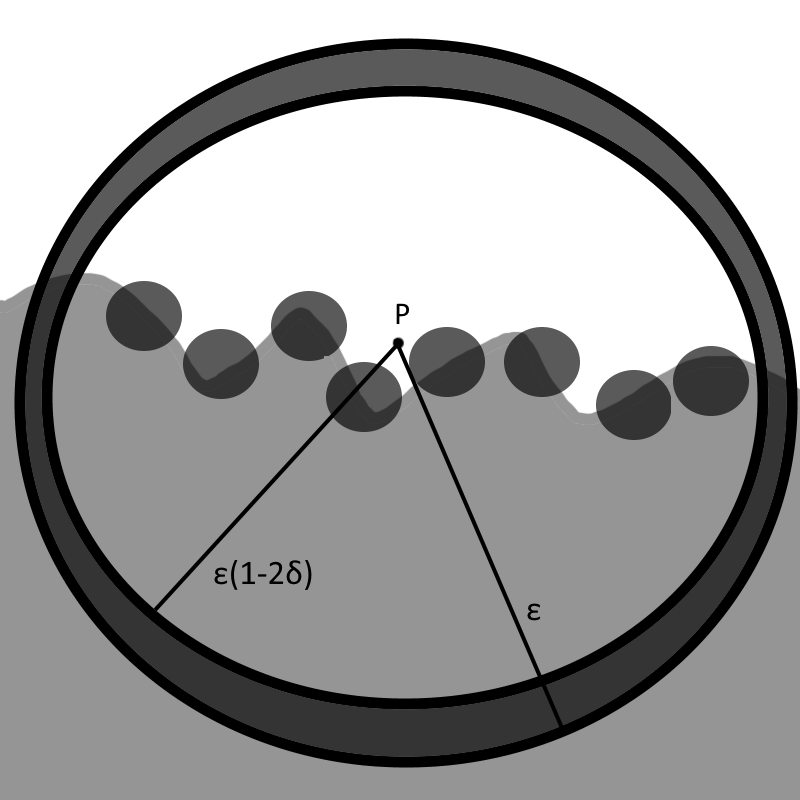
\includegraphics[width=0.4\textwidth]{covering lemma}
% \end{figure}

% \begin{sublemma}
% On $B_{1 - 2\sigma} \cap \{c\gamma^2 < \varphi < 1 - c\gamma^2\}$,
% $$(1_{V_0}(|\dif u| - Tu))_\varepsilon \lesssim_p \gamma |\dif u|_\varepsilon.$$
% \end{sublemma}
% \begin{proof}
% It follows from the definitions that for every $P \in B_\varepsilon$ and $Q \in V_0$, $\chi_\varepsilon(P - Q) \lesssim \varepsilon^{-d} \delta$,
% whence, by Proposition \ref{doubling dimension},
% \begin{align*}
% (1_{V_0}(|\dif u| - x\partial_zu))_\varepsilon &\lesssim \frac{\delta}{\varepsilon^d} \int_{B_\varepsilon} *|\dif u| \lesssim \frac{\delta}{\varepsilon}.
% \end{align*}
% Let $P \in B_\varepsilon$. Then by Lemma \ref{Giusti71}, there exists $c > 0$ such that if $\varphi \in (c\gamma^2, 1 - c\gamma^2)$, then there exists $Q \in \partial^* U$ such that $d(P, Q) < \varepsilon(1 - \gamma)$.
% If $d(Q, R) < \gamma\varepsilon/2$, then $d(P, R) < \varepsilon - \gamma\varepsilon/2$ and so $\chi_\varepsilon(P - R) \gtrsim \varepsilon^{-d}\gamma$ whenever $R \in B(Q, \gamma\varepsilon/2) =: W_0(P)$.
% We thus estimate
% $$\varepsilon^{-1} \gamma^{d - 1} \lesssim (1_{W_0(P)}|\dif u|)_\varepsilon \leq |\dif u|_\varepsilon$$
% and hence we obtain
% $$(1_{V_0}(|\dif u| - x\partial_zu))_\varepsilon(P) \lesssim \delta \gamma^{1 - d} |\dif u|_\varepsilon$$
% uniformly in $P$. Since $\delta = \gamma^d$, the claim holds.
% \end{proof}

%%%%%%%%%%%%%%%%%%%%%%%%%%%%%%%%%%%%%
\subsection{Mollification of sets of least perimeter}
We now generalize \cite[Lemma 7.5]{Giusti77}, which reduces the study of sets of least perimeter to that of sets with $C^1$ perimeter.

\begin{proposition}\label{mollifier quant}
Let $(P_n)$ be a precompact sequence in $M$ and $0 < \Delta_n \lesssim 1$.
For every $n \in \NN$ let $U_n$ be a set of least perimeter in $B_n := B(P_n, \Delta_n)$, $(x^\mu_n)$ be a normal coordinate system at $P_n$, let $T_n$ be given by (\ref{T in coords}), and 
$$\gamma_n := \Delta_n^{1 - d} \int_{B_n} \star(|\dif 1_U| - T_n 1_U).$$
If $(\gamma_n) \in \ell^1$ then for almost every $t \in (0, 1)$ and every $n \in \NN$ there exists a set $V_n$ with $C^1$ boundary in $tB_n := B(P_n, t\Delta_n)$ such that 
\begin{align}
|V_n \cap tB_n| &\leq \eta(V_n, t\Delta_n) + o(\gamma_n \Delta_n^{d - 1}), \label{mollifier quant1}\\
||U_n \cap tB_n| - |V_n \cap tB_n|| &\ll \gamma_n \Delta_n^{d - 1}, \label{mollifier quant2}\\
\lim_{n \to \infty} (\normal_{V_n}, T_n)(\Delta_n x) &= 1, \label{mollifier quant4}
\end{align}
where the limit in (\ref{mollifier quant4}) is locally uniform in $B'(0, t)$, and for every $d-1$-form $\omega_n$ defined near $P_n$,
\begin{equation}\label{mollifier quant3}
\left|\int_{tB_n} \dif(1_{U_n} - 1_{V_n}) \wedge \omega_n\right| \ll \gamma_n \Delta_n^{d - 1} ||\omega_n||_{C^1}.
\end{equation}
\end{proposition}
\begin{proof}
In this proof, we shall assume that the constants furnished by Propositions \ref{Monotonicity Formula} and \ref{main mollifier lemma} are chosen to be uniform in $n$.
This is possible because such constants are continuous in the basepoint $P$ and so can be chosen uniformly on the compact set $\overline{\{P_n: n \in \NN\}}$, and because they can be chosen uniformly in the normal coordinate system $(x^\mu)$ based at $P$.
Indeed, the moduli space of normal coordinate systems based at $P$ is just the space $\SpOrth_d$ of ordered oriented orthonormal bases of $T_PM$, which is compact.

Draw $t$ uniformly at random, let $w_n := (u_n)_{\Delta_n \gamma_n^4}$, let $c$ be as in Proposition \ref{main mollifier lemma}, and let $a_n = c\gamma_n^2$, $b_n = 1 - c\gamma_n^2$.
By the coarea formula, Proposition \ref{Coarea2},
$$\int_{tB_n} \star |\dif w_n| = \int_0^1 |\partial^* \{w_n > y\} \cap tB_n| \dif y \geq \int_{a_n}^{b_n} |\partial^* \{w_n > y\} \cap tB_n| \dif y,$$
so by the mean value theorem, there exists $y_n \in (a_n, b_n)$ such that
\begin{equation}\label{MVT mollifier}
|\partial^* \{w_n > y_n\} \cap tB_n| \leq \frac{1}{b_n - a_n} \int_{tB_n} \star |\dif w_n|.
\end{equation}
We then set $V_n := \{w_n > y_n\}$, $v_n := 1_{V_n}$, so $V_n$ has $C^1$ boundary in $tB_n$ by (\ref{claim 2 on main mollifier lemma}), and from (\ref{claim on main mollifier lemma}) and (\ref{T in coords}), on $(1 - o(1))tB_n$,
\begin{equation}\label{mollifier prop4}
g^{-1}(\dif x^1_n, \normal_{V_n}) = |\dif v_n|^{-1} g^{-1}(\dif x^1, \dif v_n) = |\dif v_n|^{-1} \sqrt{\det g_n} T_n v_n \geq (1 - o(1)) \sqrt{\det g_n}
\end{equation}
which implies (\ref{mollifier quant4}).

Let $\Gamma_n := \partial(tB_n)$; we claim that 
\begin{equation}\label{trace of vn}
||u_n - v_n||_{L^1(\Gamma_n)} \lesssim \gamma_n^{-2} ||u_n - w_n||_{L^1(\Gamma_n)} \ll \Delta_n^{d - 1} \gamma_n.
\end{equation}
To establish the claim, observe that by \cite[Lemma 7.2]{Giusti77} and Proposition \ref{doubling dimension},
$$\limsup_{n \to \infty} \Delta_n^{1 - d} \gamma_n^{-4} \int_{tB_n} \star |u_n - w_n| \leq \limsup_{n \to \infty} \Delta_n^{2-d} |\partial^* U_n \cap tB_n| \lesssim \sup_n \Delta_n \lesssim 1$$
and hence almost surely,
$$||u_n - w_n||_{L^1(\Gamma_n)} \ll \Delta_n^{d - 1} \gamma_n^3.$$
So (\ref{trace of vn}) holds by \cite[Lemma 1.25]{Giusti77} and the fact that $y_n = c\gamma_n^2$.

Let
$$f(s) = \sum_{n=1}^\infty \gamma_n \Delta_n^{1 - d} \int_{sB_n} \star |\dif u_n|.$$
Then $f' \geq 0$, and by Proposition \ref{doubling dimension}, $f(1) \lesssim \sum_n \gamma_n < \infty$.
So almost surely,
$$f(t + \gamma_n^4) - f(t) \lesssim \gamma_n^4$$
and hence
$$\int_{(t + \gamma_n^4)B_n \setminus tB_n} \star |\dif u_n| \lesssim \gamma_n \Delta_n^{d - 1}.$$
From \cite[Lemma 7.2]{Giusti77} and (\ref{MVT mollifier}) we conclude that almost surely,
\begin{equation}\label{difference of surface area}
|\partial V_n \cap tB_n| \leq |\partial^* U_n \cap tB_n| + o(\Delta_n^{d - 1} \gamma_n).
\end{equation}
Now (\ref{mollifier quant2}) follows from (\ref{trace of vn}), (\ref{difference of surface area}), and (\ref{a priori estimate 1}).
From (\ref{mollifier quant2}), (\ref{a priori estimate 1}), the fact that $U_n$ has least perimeter, and (\ref{trace of vn}), we also obtain (\ref{mollifier quant1}).

It remains to show (\ref{mollifier quant3}). Integrating by parts,
$$\left|\int_{tB_n} \dif (u_n - v_n) \wedge \omega_n\right| \leq ||\omega_n||_{L^\infty} ||u_n - v_n||_{L^1(\Gamma_n)} + ||\dif \omega_n||_{L^\infty} \int_0^1 ||u_n - v_n||_{L^1(\partial(sB_n)} \dif s.$$
The first term here is acceptable by (\ref{trace of vn}), thus 
$$\limsup_{n \to \infty} ||\omega_n||_{C^1}^{-1} \gamma_n^{-1} \Delta_n^{1 - d} \left|\int_{tB_n} \dif(u_n - v_n) \wedge \omega_n\right| \leq \limsup_{n \to \infty} \int_0^1 \gamma_n^{-1} \Delta_n^{1 - d} ||u_n - v_n||_{L^1(\partial(sB_n))} \dif s.$$
Moreover, (\ref{trace of vn}) holds with $t$ replaced by almost any $s$, so the integrand $\to 0$ almost everywhere and is uniformly in $L^\infty$.
So by Fatou's lemma, the integral is $\ll 1$.
\end{proof}



%%%%%%%%%%%%%%%%%%%%%%%%%%%%%%%%%%%%%%%%%%%%%%%

\section{Plateau's equation}\label{Plateau section}
Having shown that we can reduce the study of sets of least perimeter to sets with $C^1$ and approximately least perimeter, our next task is to represent such sets as graphs of approximate solutions to a Plateau-type equation.
It is natural to expect the Plateau equation to a PDE on a manifold $\Omega$ of dimension $d - 1$, so we now construct $\Omega$.

\subsection{Derivation}
Let $(x^\mu)$ and $\psi$ be as above, and let $\Omega \subseteq \RR^{d - 1}$ be a small open neighborhood of $0$ (on which we have not yet imposed a metric).
We introduce the projection
\begin{align*}
    \Pi: M &\to \Omega \subseteq \RR^{d - 1}\\
    x &\mapsto \overline x := (x^1, \dots, x^{d - 1}).
\end{align*}
If $\omega$ is a $C^r$ function $\Omega \to \RR$, we introduce as a section of $\Pi$ the locally closed $C^r$ embedding
\begin{align*}
    \Psi_\omega: \Omega &\to M \\
    x &\mapsto (\omega(x), x^1, x^2, \dots, x^{d - 1})
\end{align*}
which identifies $\Omega$ with the ``graph'' $N_\omega$ of $\omega$, which is a hypersurface in $M$.
We will write $y$ for $x^0$ sometimes, thus $x = (\overline x, y)$.

\begin{definition}
Let $v_1, \dots, v_{d - 1} \in T_QM$.
The \dfn{Gram form} of $v_1, \dots, v_{d - 1}$ is the quadratic form on $\spn(\partial_1, \dots, \partial_{d - 1})$ defined by
$$\Gram(v_1, \dots, v_{d - 1})_{ij} = g(v_i, v_j).$$
\end{definition}

To construct the Plateau energy, we fix $\omega: \Omega \to \RR$, and let $N = N_\omega$ be its graph.
Then $\phi_i := \dif \Psi_\omega \cdot \partial_i$ defines a tangent frame to $N$, which in coordinates is 
\begin{equation}\label{vector in frame}
\phi_i^\mu = (\dif \Psi_\omega)_\nu^\mu \delta_i^\nu = (\dif \Psi_\omega)_i^\mu = \delta^\mu_0 \omega_{,i} + \delta_i^\mu.
\end{equation}
Since $\Gram(\phi_1, \dots, \phi_{d - 1})$ is the pullback of $g|N$ to $\Omega$, we compute
$$\Gram(\phi_1, \dots, \phi_{d - 1})_{ij} = g_{00} \omega_{,i} \omega_{,j} + 2g_{i0} \omega_{,j} + g_{ij},$$
or in a more coordinate-free fashion,
\begin{equation}\label{Gram form for a frame}
\Gram(\phi_1, \dots, \phi_{d - 1}) = g_{00} (\dif \omega)^{\otimes 2} + 2g_{\hat 00} \otimes \dif \omega + g_{\hat 0\hat 0}.
\end{equation}
Thus 
\begin{align*}
\det \Gram(\phi_1, \dots, \phi_{d - 1}) &= \det(g_{00} (\dif \omega)^{\otimes 2} + 2g_{\hat 00} \otimes \dif \omega + g_{\hat 0 \hat 0}) \\
&= \det(1 + g_{\hat 0\hat 0}^{-1} g_{00} (\dif \omega)^{\otimes 2}) \cdot \det g_{\hat 0\hat 0} \cdot \det(1 + 2(g_{00} (\dif \omega)^{\otimes 2} + g_{\hat 0\hat 0})^{-1} g_{\hat 00} \otimes \dif \omega).
\end{align*}
To deal with the first factor here we shall define a family of Riemannian metrics $\slashed g(y)$, $y \in \RR$, on $\Omega$, by 
\begin{equation}\label{slashed metric}
\slashed g(y)_{ij}(\overline x) = \frac{g_{ij}(\overline x, y)}{g_{00}(\overline x, y)}
\end{equation}
where as usual $\overline x \in \Omega$ and $i,j = 1, \dots, d - 1$.
Then by the Weinstein-Aronszajn theorem,
\begin{align*}
\det(1 + g_{\hat 0\hat 0}^{-1} g_{00} (\dif \omega)^{\otimes 2}) &= \det(1 + \slashed g(\omega)^{-1} (\dif \omega)^{\otimes 2}) \\
&= 1 + |\dif \omega|_{\slashed g(\omega)^{-1}}^2.
\end{align*}
It follows from the definitions that $\Gram(\phi_1, \dots, \phi_{d - 1})_{ij}$ are the components of the metric tensor on $N$ with respect to the frame $(\phi_i)$.
Therefore, for every Borel set $E \subseteq \Omega$, one has 
$$|(\Psi_\omega)_* E| = \int_E \sqrt{\det \Gram(\phi_1(\overline x, \omega(\overline x)), \dots, \phi_{d - 1}(\overline x, \omega(\overline x)))} \dif \overline x,$$
where $\dif \overline x$ is the euclidean volume form on $\RR^{d - 1}$, so we make the following definition.

\begin{definition}\label{definition of Plateau energy}
Let $(\slashed g(y))_{y \in \RR}$ be the family of metrics on $\Omega$ defined by (\ref{slashed metric}).
Then the \dfn{Plateau energy} of a function $\omega$ and a continuous $1$-form $\sigma$ on $\Omega$ is the $d - 1$-form on $\Omega$,
\begin{equation}\label{Plateau energy}
\Lagrange[\omega, \sigma] := e^{\varphi_{\omega, \sigma}(\overline x)} \sqrt{1 + |\sigma|_{\slashed g(\omega)^{-1}}^2} \dif \overline x
\end{equation}
where $x = (\overline x, \omega(\overline x))$ and
\begin{equation}\label{Plateau error}
e^{2\varphi_{\omega, \sigma}(\overline x)} := \det g_{\hat 0\hat 0}(x) \det(1 + 2(g_{00}(x) \sigma^{\otimes 2}(\overline x) + g_{\hat 0\hat 0}(x))^{-1} g_{\hat 00}(x) \otimes \sigma(\overline x)).
\end{equation}
The \dfn{Plateau equation} is the Euler-Lagrange equation for $\Lagrange$.
\end{definition}

From the discussion prior to Definition \ref{definition of Plateau energy} we have the following:

\begin{proposition}\label{construction of Plateau energy}
For $N = N_\omega$, $\omega \in C^1(\Omega)$, the Plateau energy $\Lagrange[\omega, \dif \omega]$ is the pullback by $\Psi_\omega$ of the volume form on $N$.
In particular, $N$ is a nonparametric minimal hypersurface iff $\omega$ is a minimizer of $\int \Lagrange[\omega, \dif \omega]$.
\end{proposition}

\begin{corollary}\label{C1 implies smooth}
Let $U$ be a set of least perimeter. If $\normal_U$ extends to a continuous $1$-form on $\partial U$, then $\partial U$ is a smooth minimal hypersurface.
\end{corollary}
\begin{proof}
By Proposition \ref{locality of Caccioppoli}, $\partial U$ is a $C^1$ minimal hypersurface.
Selecting appropriate normal coordinate charts centered on $\partial U$, we realize $\partial U$ locally as the graph of a $C^1$ function $\omega$ which is a weak solution of the Plateau equation by Proposition \ref{construction of Plateau energy}.
Therefore $\omega$ is smooth (see \cite[\S8.3.2]{evans2010partial} and the references therein).
\end{proof}

%%%%%%%%%%%%%%%%%%%%%%%%%%%%%%%%%%%%%%%%
\subsection{The conormal $1$-form}
It follows from Corollary \ref{C1 implies smooth} that $\normal_U$ is now of interest when $U$ is a set of least perimeter, so we turn to a study of a such $1$-forms.

\begin{definition}
The \dfn{cross product} $v_1 \times \cdots \times v_{d - 1}$ of vectors $v_1, \dots, v_{d - 1} \in T_QM$ is the unique vector $v_0$
such that:
\begin{enumerate}
\item $g(v_0, v_i) = 0$,
\item $((-1)^{d - 1} v_0, v_1, \dots, v_{d - 1})$ is positively oriented or linearly dependent, and
\item $g(v_0, v_0) = |\det \Gram(v_1, \dots, v_{d - 1})|$.
\end{enumerate}
\end{definition}

\begin{lemma}
Let $\omega$ and $\phi_i = \dif \Psi_\omega \cdot \partial_i$ be as above.
The cross product $\phi_0 := \phi_1 \times \cdots \phi_{d - 1}$ is 
\begin{equation}\label{phi0 components}
\phi_0^\mu = e^{O(|x|^2 + |\omega(x)|^2)} (g^{\mu 0} + g^{\mu i}\omega_{,i}).
\end{equation}
\end{lemma}


\begin{proposition}
The conormal $1$-form to $N = N_\omega$ is
\begin{equation}\label{conormal}
\normal_\mu(x, \omega(x)) = \frac{e^{O(|x|^2 + |\omega(x)|^2)}}{\sqrt{1 + |\dif \omega(x)|^2_{(\slashed g^{(\omega(x))})^{-1}(x)}}} (\delta^0_\mu - \delta^i_\mu \partial_i \omega(x)).
\end{equation}
\end{proposition}
\begin{proof}
It is clear from (\ref{definition of slashed g}) that (\ref{decay of slashed metric}) holds.
Moreover, if we let
$$h_{ij} = g(\phi_i, \phi_j)$$
be the pullback by $\Psi_\omega$ of the Riemannian metric on $N_\omega$, then $h = \Gram(\phi_1, \dots, \phi_{d - 1})$ and so
$$\Lagrange[\omega, \grad_{\slashed g} \omega] = \Psi_\omega^* |\phi_0|_{\slashed g^{(\omega)}} \dif x^1 \wedge \cdots \wedge \dif x^{d - 1}$$
which gives the formula (\ref{Plateau energy}).

Finally, it follows from the definition of cross product that $\normal = \phi_0/|\phi_0|$.
We therefore claim that

which implies (\ref{conormal}). To prove (\ref{phi0 components}) we observe that $\phi_0$ depends smoothly on $g$ and so if we replace $g$ with the metric $g'$ defined by $g'_{00} = g_{00}$, $g'_{ij} = g_{ij}$, $g'_{0i} = 0$, then it suffices to show that the new cross product $\phi_0'$ satisfies
\begin{equation}\label{perturbed phi0 components}
(\phi_0')^\mu = g^{\mu\nu}(\delta_\nu^0 - \delta_\nu^i\omega_{,i}).
\end{equation}
With $g$ replaced by $g'$ we obtain the exact formula
\begin{equation}\label{perturbed norm of phi0}
g(\phi_0', \phi_0') = \sqrt{\det \slashed g} \sqrt{1 + |\dif \omega|_{\slashed g^{(\omega)}}}
\end{equation}
in place of (\ref{norm of phi0}), and so we just need to show that if $\phi_0'$ satisfies (\ref{perturbed phi0 components}) then it is $g'$-orthogonal to the span of $\phi_1, \dots, \phi_{d - 1}$ and has norm (\ref{perturbed norm of phi0}).
Orthogonality follows from the computation
$$g'(\phi_0', \phi_i) = g'_{\mu\nu} (\phi_0')\mu \phi_i^\nu = \delta_\mu^\nu (\delta_0^\mu \omega_{,i} + \delta_i^\mu) (\delta_\nu^0 - \delta_\nu^i \omega_{,i}) = 0.$$
To prove (\ref{perturbed norm of phi0}) we just compute
\begin{align*}
g'(\phi_0', \phi_0')
&= g'_{\mu \nu} (g')^{\mu \lambda}(\delta^0_\lambda - \delta^i_\lambda \omega_{,i}) (g')^{\nu \kappa}(\delta_\kappa^0 - \delta_\kappa^j \omega_{,j})\\
&= (\delta_\mu^0 - \delta_\nu^i \omega_{,i})((g')^{0 \nu} - (g')^{j \nu} \omega_{,j})\\
&= (g')^{00} - (g')^{0j} \omega_{,j} - (g')^{0i} \omega_{,i} + (g')^{ij} \omega_{,i} \omega_{,j}.
\end{align*}
From the definition of $g'$ we can rewrite this last expression as
$$g'(\phi_0', \phi_0') = (g_{00})^{-1} + (g_{\hat 0 \hat 0})^{-1} \dif \omega^{\otimes 2}.$$
But $g_{00} (g_{\hat 0 \hat 0})^{-1} = \slashed g^{-1}$ so this is as desired.
\end{proof}

%%%%%%%%%%%%%%%%%%%%%%%%%%%%%%%%%%%%%%%%%%%%%%%%%%%%%%%%%%%%%
\subsection{A multiplicative gain}
We now apply the strategy of Miranda \cite[Teorema 4.3]{Miranda66} to obtain a multiplicative gain on the mean oscillation of the Plateau energy $\Lagrange[\omega, \grad_{\slashed g} \omega]$ when one passes from a dyadic scale $r$ to its child $r/2$.
To motivate why the same argument should work in our context, we note that the result of Miranda is effective when $|\grad \omega| \ll 1$.
So we shall linearize the Plateau equation about the constant solution $\omega = \omega(0)$.
From the expansion (\ref{decay of slashed metric}), we can then replace $\slashed g^{(y)}$ with the euclidean metric. Taylor expanding (\ref{Plateau energy}) to second order in $\grad \omega$ and approximating $e^{O(|x|^2)}$ by $1$, we arrive at the \dfn{Dirichlet energy}
$$\DirL[\grad \omega] := \frac{1}{2} |\grad \omega|^2,$$
whose Euler-Lagrange equation is the euclidean Laplace equation, just as in the argument of Miranda.

We shall need the following notation.
Let $\tilde B_r$ denote the euclidean ball centered on $0$ of radius $r$, thus $\tilde B_r = \Pi(B_r)$.
For a tensor field $T$, let
$$(\avg_r T)_{ij} = \dashint_{\tilde B_r} T_{ij}(x) \dif x,$$
which defines a constant tensor field on $\RR^{d - 1}$ (this makes sense because the Levi-Civita connection on $\RR^{d - 1}$ is flat).
For an open set $\Omega \subseteq \RR^{d - 1}$, we identify $\Omega \times \RR$ with a subset of $M$ and endow it with the metric $g$.
We identify Lagrangians with their euclidean Hodge duals, and suppress the $(\cdot)^{-1}$s that indicate that we are working with the cometric.

\begin{proposition}\label{dGL Laplace}
Let $0 \in \Omega \subseteq \RR^{d - 1}$. For every $c > 0$ there exists $r^* = r^*(c) > 0$ such that for every $\omega \in C^1(\Omega)$ such that $\omega(0) = 0$, $0 < \kappa, \beta < 1$, and $0 < r < r^*$, if
\begin{align}
||\dif \omega||_{L^\infty(B_r)} &\leq \kappa \label{bound on gradient}, \\
\int_{\tilde B_r} \Lagrange[\omega, \dif \omega] - \Lagrange[\omega, \avg_r \dif \omega] &\leq \beta, \label{bound on mean oscillation} \\
\int_{\tilde B_r} \Lagrange[\omega, \dif \omega] - \eta(\{(x, y): y < \omega(x)\}, 2^{-n}) &\leq \beta\kappa \label{bound on surface area},
\end{align}
then
\begin{equation} \label{dGL Laplace gain}
\int_{\tilde B_{r/2}} \Lagrange[\omega, \dif \omega] - \Lagrange[\omega, \avg_{r/2} \dif \omega] \leq e^{O(c)}\left(\frac{\beta}{2^{d + 1}} + O_c(\beta \sqrt \kappa) + O_c(r^{-d} \kappa)\right).
\end{equation}
\end{proposition}
\begin{proof}
We follow \cite[Lemma 4.2]{Miranda66}, but with modifications to account for the additional nonlinearities and lack of constant coefficients in the Lagrangian $\Lagrange[\omega, \dif \omega]$.

Since $\omega(0) = 0$, $|\omega(x)| = O(|x|)$. Thus if $r$ is small enough depending on $c$, we have from (\ref{Plateau energy}) and Taylor's theorem that
\begin{align*}
\Lagrange(\omega, \dif \omega) - \Lagrange(\omega, \avg_{r/2} \dif \omega)
\leq \frac{e^c}{2} \left[|\dif \omega|_{\slashed g^{(\omega)}}^2 - |\avg_{r/2} \dif \omega|_{\slashed g^{(\omega)}}^2\right].
\end{align*}
Letting $b^{ij} = ((\slashed g^{(\omega)})^{ij} - \delta^{ij})/2$ we obtain $b^{ij} = O(|x|^2)$ and
$$\Lagrange(\omega, \dif \omega) - \Lagrange(\omega, \avg_{r/2} \dif \omega) \leq e^c\left(\DirL(\dif \omega) - \DirL(\avg_{r/2} \dif \omega) + b^{ij} \avg_{r/2} \omega_{,i} \avg_{r/2} \omega_{,j} - b^{ij} \omega_{,i} \omega_{,j}\right).$$
Moreover one has
$$\int_{\tilde B_{r/2}} b^{ij} \avg_{r/2} \omega_{,i} \avg_{r/2} \omega_{,j} - b^{ij} \omega_{,i} \omega_{,j} \lesssim ||\dif \omega||_{L^\infty(\tilde B_r)}^2 \int_0^{r/2} s^2 |\partial \tilde B_s| \dif s \lesssim \kappa^2 r^{d + 1}.$$
We can therefore estimate
$$\int_{\tilde B_{r/2}} \Lagrange[\omega, \dif \omega] - \Lagrange[\omega, \avg_{r/2} \dif \omega] \leq e^c \int_{\tilde B_{r/2}} \DirL[\dif \omega] - \DirL[\avg_{r/2} \dif \omega] + O(\kappa^2 r^{d + 1}).$$

Let $h$ be the harmonic function on $\tilde B_r$ such that $h = \omega$ on $\partial \tilde B_r$.
By definition of $\eta$ and (\ref{bound on surface area}),
\begin{equation}\label{bounds on the harmonic}
\int_{\tilde B_{r/2}} \Lagrange[\omega, \dif \omega] - \Lagrange[\omega, \dif h] \leq \int_{\tilde B_r} \Lagrange[\omega, \dif \omega] - \eta(\{(x, y): y < \omega(x)\}, 2^{-n}) \leq \beta \kappa.
\end{equation}
By definition of $\avg_{r/2} \dif \omega$, for every $\varepsilon > 0$ small,
\begin{align*}
\int_{\tilde B_{r/2}} \DirL[\dif \omega] - \DirL[\avg_{r/2} \dif \omega]
&\leq \int_{\tilde B_{r/2}} \DirL[\dif \omega - \avg_r \dif\omega] \\
&\leq (1 + \varepsilon^{-1}) \int_{\tilde B_{r/2}} \DirL[\dif (\omega - h)] +(1 + \varepsilon) \int_{\tilde B_{r/2}} \DirL[\dif h - \avg_r \dif \omega] \\
&=: O(\varepsilon^{-1}) I_1 + (1 + \varepsilon) I_2.
\end{align*}
From the positivity of Dirichlet energy and the mean value property of $h$,
$$I_1 = \int_{\tilde B_{r/2}} \DirL[\dif (\omega - h)] \leq \int_{\tilde B_r} \DirL[\dif \omega] - \DirL[\dif h]$$
and from Taylor expansion of $\Lagrange[\omega, \cdot]$ and (\ref{bounds on the harmonic}) we have TODO seems sus
$$\int_{\tilde B_r} \DirL[\dif \omega] - \DirL[\dif h] \lesssim \int_{\tilde B_r} \Lagrange[\omega, \dif \omega] - \Lagrange[\omega, \dif h] \leq \beta \kappa.$$
Applying \cite[Lemma 4.1]{Miranda66} as in the proof of \cite[Lemma 4.2]{Miranda66} we have
$$I_2 \leq (1 + \varepsilon) 2^{-(d + 1)} \int_{\tilde B_r} \DirL[\dif \omega - \avg_r \dif \omega] + O(\varepsilon^{-1}) I_1;$$
the latter term is of course $O(\beta \kappa/\varepsilon)$.

\end{proof}

%%%%%%%%%%%%%%%%%%%%%%%%%%%%%%%%%%%%%%

\section{Regularity of minimal hypersurfaces}\label{de Giorgi section}
\subsection{Excess: first properties}
\subsection{Excess and Plateau's equation}
\subsection{de Giorgi's lemma}
\begin{proposition}[de Giorgi's lemma]\label{dGL final}
hello
\end{proposition}
\subsection{Induction on scale}


\printbibliography

\end{document}
